% Compile with XeLaTeX; see README.md.
\documentclass[12pt,a4paper,oneside,openany]{book}
\usepackage{fontspec}
\setmainfont{Times New Roman}
\setsansfont{Arial}
\setmonofont{Consolas}[Scale=MatchLowercase]
\usepackage{hcmus-report-template-book}
\usepackage{booktabs,tabularx,longtable,needspace,bookmark}
\geometry{top=2.2cm,bottom=2.2cm,left=2.5cm,right=2cm}
\setlength{\parindent}{0pt}
\setlength{\parskip}{5pt plus 1pt}
\setstretch{1.25}
\setlength{\emergencystretch}{3em}
\setlength{\headheight}{16pt}
\setlength{\headsep}{14pt}
\setlength{\tabcolsep}{6pt}
\renewcommand{\arraystretch}{1.2}
\setlength{\arrayrulewidth}{0.4pt}
\raggedbottom
\widowpenalty=10000
\clubpenalty=10000
\hypersetup{unicode=true,colorlinks=true,linkcolor=black,citecolor=black,urlcolor=black,
  pdftitle={Báo cáo học phần Lịch sử Đảng Cộng sản Việt Nam},
  pdfauthor={Nhóm 3 - Lớp 23C02},
  pdfsubject={Từ đường lối đến thực tiễn: học liệu lịch sử 1954--1975},bookmarksnumbered=true}
\addto\captionsvietnamese{
  \renewcommand{\chaptername}{Phần}
  \renewcommand{\contentsname}{MỤC LỤC}
  \renewcommand{\listfigurename}{DANH MỤC HÌNH ẢNH}
  \renewcommand{\listtablename}{DANH MỤC BẢNG}
  \renewcommand{\bibname}{TÀI LIỆU THAM KHẢO}}
\titleformat{\chapter}[display]{\normalfont\bfseries}
  {\large PHẦN \thechapter}{6pt}{\LARGE}
\titlespacing*{\chapter}{0pt}{0pt}{18pt}
\titleformat{\section}{\large\bfseries}{\thesection.}{0.6em}{}
\titleformat{\subsection}{\normalsize\bfseries}{\thesubsection.}{0.6em}{}
\titlespacing*{\section}{0pt}{12pt}{5pt}
\titlespacing*{\subsection}{0pt}{9pt}{4pt}
\setcounter{tocdepth}{1}
\setcounter{secnumdepth}{2}
\captionsetup{font=small,labelfont=bf,labelsep=period,skip=6pt}
\captionsetup[table]{position=bottom}
\setlength{\textfloatsep}{14pt plus 2pt minus 2pt}
\setlength{\intextsep}{12pt plus 2pt minus 2pt}
\newcolumntype{L}{>{\raggedright\arraybackslash}X}
\newcommand{\coursename}{Lịch sử Đảng Cộng sản Việt Nam}
\newcommand{\reporttitle}{TỪ ĐƯỜNG LỐI ĐẾN THỰC TIỄN}
\newcommand{\reportname}{Tìm hiểu sự lãnh đạo của Đảng trong kháng chiến chống Mỹ, cứu nước (1954--1975)}
\newcommand{\studentname}{Nhóm 3}
\newcommand{\teachername}{ThS. Trần Thị Châu}
\fancypagestyle{report}{
  \fancyhf{}
  \fancyhead[L]{\small Báo cáo học phần Lịch sử Đảng}
  \fancyhead[R]{\small Nhóm 3 -- Lớp 23C02}
  \fancyfoot[C]{\small\thepage}
  \renewcommand{\headrulewidth}{0.3pt}}
\fancypagestyle{plain}{
  \fancyhf{}\fancyfoot[C]{\small\thepage}\renewcommand{\headrulewidth}{0pt}}
\begin{document}
\selectlanguage{vietnamese}
\frontmatter
\pagestyle{plain}
\begin{titlepage}
\centering
\thispagestyle{empty}
{\large ĐẠI HỌC QUỐC GIA THÀNH PHỐ HỒ CHÍ MINH\par}
\vspace{0.15cm}
{\Large\bfseries TRƯỜNG ĐẠI HỌC KHOA HỌC TỰ NHIÊN\par}

\includegraphics[width=8cm]{img/hcmus-logo.png}\par
{\large\bfseries BÁO CÁO SẢN PHẨM\par}
{\large\coursename\par}
\vspace{0.45cm}
{\rule{0.9\linewidth}{0.7pt}\par}
\vspace{0.35cm}
{\LARGE\bfseries\reporttitle\par}
\vspace{0.35cm}
\begin{minipage}{0.92\linewidth}
\centering
{\Large\bfseries\reportname\par}
\vspace{0.35cm}
{\large Góc nhìn từ chứng tích lịch sử tại\\Bảo tàng Chứng tích Chiến tranh\par}
\vspace{0.35cm}
\end{minipage}\par
\vspace{0.45cm}
{\rule{0.9\linewidth}{0.7pt}\par}
{\large\studentname\ - Lớp 23C02\par}
{\large Giảng viên: \teachername\par}
\vfill
{\large Thành phố Hồ Chí Minh, tháng 11 năm 2026\par}
\end{titlepage}

\pagenumbering{Roman}
\chapter*{THÀNH VIÊN NHÓM 3}
\addcontentsline{toc}{chapter}{Thành viên nhóm 3}
\noindent\textbf{Lớp:} 23C02\\
\textbf{Học phần:} Lịch sử Đảng Cộng sản Việt Nam\par
\begin{table}[H]
\centering
\begingroup
\small
\setstretch{1.15}
\setlength{\tabcolsep}{4pt}
\renewcommand{\arraystretch}{1.5}
\setlength{\extrarowheight}{4pt}
\begin{tabularx}{\textwidth}{|>{\centering\arraybackslash}m{0.8cm}|m{4.15cm}|>{\centering\arraybackslash}m{2cm}|L|}
\hline
\textbf{STT} & \textbf{Họ và tên} & \textbf{MSSV} & \textbf{Nhiệm vụ chính} \\
\hline
1 & Lê Nguyễn Nhật Trường & 23127136 & Nhóm trưởng; điều phối tiến độ và tổng hợp báo cáo. \\
\hline
2 & Biện Xuân An & 23127020 & Nội dung giai đoạn 1969--1973 và Hiệp định Paris. \\
\hline
3 & Đoàn Lê Gia Bảo & 23127025 & Nội dung giai đoạn 1954--1960 và phong trào Đồng Khởi. \\
\hline
4 & Hoàng Minh Giang & 23127043 & Xây dựng giao diện chung và dòng thời gian tương tác. \\
\hline
5 & Lê Hữu Minh Quang & 23127108 & Biên soạn tổng kết, bộ câu hỏi ôn tập và hiệu đính nội dung. \\
\hline
6 & Văn Ngọc Quý & 23127114 & Xây dựng kho tư liệu và giao diện xem chi tiết hiện vật. \\
\hline
7 & Mạch Quốc Tấn & 23127115 & Nội dung giai đoạn 1973--1975 và Chiến dịch Hồ Chí Minh. \\
\hline
8 & Nguyễn Văn An & 23127317 & Nội dung giai đoạn 1965--1968 và Tết Mậu Thân. \\
\hline
9 & Vũ Hoàng Minh & 23127427 & Xây dựng phần trắc nghiệm và trang nhóm tác giả. \\
\hline
10 & Vương Khải Phong & 23127453 & Nội dung giai đoạn 1961--1965 và chiến lược ``Chiến tranh đặc biệt''. \\
\hline
\end{tabularx}
\endgroup
\caption{Danh sách thành viên và phân công nhiệm vụ}
\label{tab:members}
\end{table}
\vspace{0.3cm}
\noindent\textbf{Sản phẩm học liệu số:}\\
\url{https://nhom03-lsd-23c02.vercel.app/}
\clearpage

\begingroup
\setstretch{1.05}
\tableofcontents
\listoffigures
\begingroup
\let\clearpage\relax
\listoftables
\endgroup
\endgroup
\mainmatter
\pagestyle{report}
% Generated by prepare_content.py from the accepted Markdown report.
\chapter{MỞ ĐẦU}

\section{Lý do xây dựng website học liệu}

Việc học tập môn Lịch sử Đảng Cộng sản Việt Nam không chỉ đòi hỏi ghi nhớ các mốc thời gian mà còn cần hiểu mối quan hệ giữa bối cảnh lịch sử, đường lối lãnh đạo và kết quả thực tiễn. Đối với giai đoạn kháng chiến chống Mỹ, cứu nước từ năm 1954 đến năm 1975, lượng kiến thức trải dài qua nhiều thời kỳ, gắn với những chuyển biến về nhiệm vụ chiến lược và phương pháp đấu tranh. Điều này đặt ra nhu cầu tổ chức kiến thức thành một hệ thống rõ ràng, thuận tiện cho việc tìm hiểu, đối chiếu và ôn tập.

Từ nhu cầu đó, nhóm lựa chọn xây dựng website học liệu với chủ đề “Từ đường lối đến thực tiễn”. Website là sản phẩm chính của đề tài, kết hợp nội dung lịch sử theo năm giai đoạn với dòng thời gian tương tác, tư liệu minh họa và câu hỏi trắc nghiệm. Thay vì tiếp cận các sự kiện như những thông tin riêng lẻ, người học có thể theo dõi tiến trình, tìm hiểu từng giai đoạn và tự kiểm tra kiến thức trên cùng một giao diện.

Việc liên hệ với chứng tích tại Bảo tàng Chứng tích Chiến tranh bổ sung góc nhìn trực quan cho học liệu. Những hiện vật, hình ảnh và nội dung trưng bày giúp kết nối kiến thức trong giáo trình với điều kiện chiến đấu, đời sống nhân dân và hậu quả của chiến tranh. Hướng tiếp cận này góp phần làm rõ ý nghĩa của các chủ trương lịch sử, đồng thời bồi dưỡng thái độ trân trọng hòa bình và trách nhiệm của thế hệ trẻ.

Là sinh viên Trường Đại học Khoa học Tự nhiên, nhóm mong muốn vận dụng khả năng ứng dụng công nghệ thông tin để tạo ra một công cụ hỗ trợ học tập phù hợp với học phần. Sản phẩm hướng tới việc trình bày kiến thức có chọn lọc, dễ theo dõi và có sự tương tác của người sử dụng. Giáo trình giữ vai trò nền tảng học thuật; website hỗ trợ hệ thống hóa, minh họa và ôn tập, không thay thế việc nghiên cứu tài liệu chính của môn học.

\section{Mục tiêu và nhiệm vụ xây dựng sản phẩm}

\textbf{Mục tiêu tổng quát} là xây dựng một website học liệu tương tác về sự lãnh đạo của Đảng trong cuộc kháng chiến chống Mỹ, cứu nước giai đoạn 1954 - 1975, phục vụ việc tìm hiểu và ôn tập của sinh viên. Nội dung được tổ chức theo hướng kết nối đường lối với thực tiễn, kết hợp kiến thức từ giáo trình với tư liệu chứng tích lịch sử.

\textbf{Mục tiêu cụ thể} gồm ba phương diện. Về nội dung, website hệ thống hóa những kiến thức trọng tâm, làm rõ sự phát triển của đường lối qua từng giai đoạn. Về cách tiếp cận, sản phẩm tạo điều kiện để người học chủ động lựa chọn nội dung, quan sát tư liệu và kiểm tra mức độ ghi nhớ. Về giáo dục, học liệu hướng tới việc bồi dưỡng nhận thức lịch sử, lòng biết ơn và ý thức trách nhiệm đối với cộng đồng, đất nước.

Để thực hiện các mục tiêu trên, nhóm xác định những nhiệm vụ sau:

\begin{enumerate}
\item Hệ thống hóa nội dung theo năm giai đoạn: 1954 - 1960, 1961 - 1965, 1965 - 1968, 1969 - 1973 và 1973 - 1975; mỗi giai đoạn làm rõ bối cảnh, chủ trương của Đảng, kết quả thực tiễn và kiến thức cần ghi nhớ.
\item Tổ chức nội dung dưới dạng trình chiếu kết hợp dòng thời gian tương tác, cho phép người học chuyển giữa các giai đoạn và theo dõi tiến trình lịch sử.
\item Xây dựng khu vực tư liệu chứng tích, gắn hình ảnh và phần giới thiệu với giai đoạn liên quan; gắn tư liệu với thời kỳ tương ứng và hỗ trợ xem thông tin chi tiết.
\item Xây dựng phần trắc nghiệm ôn tập với phản hồi đúng, sai, giải thích đáp án và kết quả làm bài để hỗ trợ người học tự kiểm tra kiến thức.
\item Tổng hợp vai trò lãnh đạo của Đảng, nguyên nhân thắng lợi, ý nghĩa lịch sử và bài học kinh nghiệm để giúp người học liên kết kiến thức giữa các giai đoạn.
\item Tổ chức giao diện và điều hướng thống nhất giữa các khu vực, bảo đảm mối liên hệ giữa hoạt động đọc học liệu, xem tư liệu và ôn tập.
\end{enumerate}

\section{Đối tượng sử dụng và phạm vi sản phẩm}

\textbf{Đối tượng sử dụng chủ yếu} là sinh viên học môn Lịch sử Đảng Cộng sản Việt Nam, đặc biệt những người cần hệ thống hóa kiến thức về giai đoạn 1954 - 1975. Website cũng được định hướng làm phương tiện minh họa khi thảo luận hoặc trình bày nội dung học tập theo nhóm.

\textbf{Về nội dung}, học liệu tập trung vào sự lãnh đạo của Đảng trong kháng chiến chống Mỹ, cứu nước, gắn nhiệm vụ xây dựng miền Bắc với đấu tranh giải phóng miền Nam. Các sự kiện được lựa chọn nhằm làm rõ mối quan hệ giữa bối cảnh, đường lối và thực tiễn, không đặt mục tiêu tái hiện toàn bộ diễn biến chiến tranh. Việc phân chia thành năm giai đoạn phục vụ tổ chức kiến thức và điều hướng trên website.

\textbf{Về nguồn tài liệu}, sản phẩm sử dụng \emph{Giáo trình Lịch sử Đảng Cộng sản Việt Nam} do Bộ Giáo dục và Đào tạo tổ chức biên soạn, Nhà xuất bản Chính trị quốc gia Sự thật xuất bản năm 2021 làm cơ sở học thuật chính. Trọng tâm là phần lãnh đạo xây dựng chủ nghĩa xã hội ở miền Bắc và kháng chiến chống Mỹ, cứu nước trong Chương 2. Tư liệu từ Bảo tàng Chứng tích Chiến tranh được sử dụng để liên hệ, minh họa cho nội dung lịch sử. [1, tr. 180 - 235].

\textbf{Về chức năng}, website tập trung vào ba hoạt động: tìm hiểu kiến thức qua trình chiếu và dòng thời gian; xem tư liệu chứng tích theo giai đoạn; tự ôn tập bằng trắc nghiệm có giải thích. Phần tổng kết và bài học hỗ trợ khái quát nội dung, còn phần giới thiệu nhóm cung cấp thông tin về tập thể thực hiện sản phẩm.

\textbf{Về giá trị sử dụng}, sản phẩm được định hướng hỗ trợ tự học và trình bày kiến thức trong phạm vi học phần. Kết quả trắc nghiệm phản ánh mức độ trả lời đúng đối với bộ câu hỏi của website, không thay thế đánh giá chính thức của giảng viên.

\section{Phương pháp thực hiện}

\textbf{Nghiên cứu và chọn lọc nội dung} được tiến hành trên cơ sở giáo trình, kết hợp phương pháp lịch sử và phương pháp logic. Các sự kiện được đặt theo trình tự thời gian và trong hoàn cảnh cụ thể; đồng thời làm rõ quan hệ giữa mục tiêu, chủ trương, tổ chức thực hiện và kết quả. Đây là cơ sở để lựa chọn kiến thức phù hợp với chủ đề của website.

\textbf{Biên soạn học liệu số} được thực hiện bằng cách phân tích, tổng hợp và chuyển nội dung nghiên cứu thành những đơn vị kiến thức ngắn gọn. Các giai đoạn sử dụng chung một cấu trúc trình bày để thuận tiện theo dõi và so sánh. Nội dung tổng kết kết nối các giai đoạn, trong khi câu hỏi ôn tập tập trung vào những luận điểm và sự kiện trọng tâm.

\textbf{Khai thác tư liệu trực quan} kết hợp hiện vật, ảnh tư liệu, nội dung giới thiệu của bảo tàng và ghi nhận khảo sát của các thành viên. Tư liệu được xem xét theo nguồn gốc, bối cảnh và nội dung phản ánh trước khi liên hệ với kiến thức lịch sử. Cách thực hiện này giúp hình ảnh giữ vai trò bổ trợ cho nhận thức, thay vì chỉ làm yếu tố trang trí.

\textbf{Tổ chức trải nghiệm học tập trên website} dựa trên mối liên hệ giữa đọc, quan sát và tự kiểm tra. Dòng thời gian hỗ trợ định vị giai đoạn; khu vực trình chiếu trình bày kiến thức; kho tư liệu bổ sung hình ảnh và thông tin; phần trắc nghiệm đưa ra phản hồi cùng giải thích. Các khu vực được kết nối bằng hệ thống điều hướng để người học chủ động lựa chọn nội dung phù hợp với nhu cầu.

\textbf{Rà soát sản phẩm} tập trung vào sự nhất quán giữa nội dung lịch sử, chú thích tư liệu, câu hỏi và đáp án, cùng cách hiển thị và điều hướng giữa các khu vực. Tiêu chí xem xét là mức độ rõ ràng của học liệu, khả năng thực hiện các thao tác cơ bản và sự phù hợp với mục tiêu hỗ trợ học tập của môn học.

\clearpage

% Nội dung báo cáo được chuyển từ bản Markdown đã đối chiếu.
\chapter{NỘI DUNG NGHIÊN CỨU QUA NĂM GIAI ĐOẠN LỊCH SỬ}

\section{Giai đoạn 1954 đến 1960}

\subsection{Bối cảnh lịch sử}

Sau Hiệp định Giơ-ne-vơ năm 1954, miền Bắc được giải phóng, trong khi đất nước tạm thời bị chia cắt. Nhiệm vụ hòa bình, thống nhất chưa hoàn thành. Miền Bắc bước vào khôi phục kinh tế, hàn gắn hậu quả chiến tranh và từng bước xây dựng cơ sở cho chủ nghĩa xã hội. Ở miền Nam, Mỹ từng bước thay thế vai trò của Pháp, hậu thuẫn chính quyền Ngô Đình Diệm, chống lại việc thực hiện tổng tuyển cử thống nhất đất nước. [1, tr. 180 - 183].

Các hoạt động “tố cộng, diệt cộng”, bắt bớ và đàn áp làm lực lượng cách mạng miền Nam chịu nhiều tổn thất. Thực tiễn đặt ra yêu cầu vừa giữ gìn cơ sở, vừa tìm phương thức đấu tranh phù hợp để bảo vệ nhân dân và duy trì phong trào. Chính trong bối cảnh đó, việc điều chỉnh phương pháp đấu tranh trở thành yêu cầu cấp thiết của cách mạng miền Nam. [1, tr. 186 - 192].

\subsection{Chủ trương và đường lối của Đảng}

Sau năm 1954, Đảng xác định nhiệm vụ củng cố miền Bắc, đấu tranh thực hiện Hiệp định Giơ-ne-vơ và giữ gìn lực lượng cách mạng ở miền Nam. Trong điều kiện mới, yêu cầu bảo vệ hòa bình gắn với việc chuẩn bị lực lượng lâu dài, không tách nhiệm vụ của từng miền khỏi mục tiêu chung của cả nước.

Hội nghị Trung ương 15 năm 1959 là bước chuyển quan trọng về phương pháp cách mạng miền Nam. Trung ương xác định con đường cơ bản là khởi nghĩa giành chính quyền về tay nhân dân, dựa vào sức mạnh chính trị của quần chúng, kết hợp với lực lượng vũ trang. Chủ trương này đáp ứng yêu cầu bức thiết của phong trào, mở ra khả năng kết hợp đấu tranh chính trị với đấu tranh vũ trang thay vì chỉ dựa vào một hình thức đơn lẻ. [1, tr. 190 - 191].

Đại hội đại biểu toàn quốc lần thứ III của Đảng tháng 9/1960 xác định tiến hành đồng thời cách mạng xã hội chủ nghĩa ở miền Bắc và cách mạng dân tộc dân chủ nhân dân ở miền Nam. Miền Bắc giữ vai trò quyết định nhất đối với sự phát triển của cách mạng cả nước; miền Nam giữ vai trò quyết định trực tiếp đối với sự nghiệp giải phóng miền Nam. Hai nhiệm vụ có quan hệ chặt chẽ, cùng hướng tới hòa bình và thống nhất Tổ quốc. Đây là cơ sở chiến lược để xây dựng hậu phương, phát triển tiền tuyến và huy động sức mạnh cả nước trong những giai đoạn tiếp theo. [1, tr. 193 - 195].

\subsection{Kết quả thực tiễn và ý nghĩa}

Phong trào Đồng Khởi năm 1959 - 1960, tiêu biểu tại Bến Tre ngày 17/1/1960, thể hiện sự phát triển của phong trào quần chúng khi đấu tranh chính trị kết hợp với đấu tranh vũ trang. Những cuộc nổi dậy làm suy yếu bộ máy kiểm soát ở nhiều vùng nông thôn, mở rộng quyền làm chủ của nhân dân và tạo bước chuyển từ thế giữ gìn lực lượng sang thế tiến công. Vai trò của phụ nữ và lực lượng đấu tranh chính trị cho thấy sức mạnh cách mạng không chỉ nằm ở hoạt động quân sự.

Ngày 20/12/1960, Mặt trận Dân tộc Giải phóng miền Nam Việt Nam ra đời, tạo hình thức tổ chức để tập hợp rộng rãi các lực lượng yêu nước. Những chuyển biến này cho thấy mối liên hệ giữa chủ trương đúng với khả năng tổ chức nhân dân thực hiện; đồng thời tạo tiền đề để cách mạng miền Nam đối phó với chiến lược “Chiến tranh đặc biệt” từ năm 1961. [1, tr. 191 - 192].

\subsection{Liên hệ chứng tích lịch sử}

Chứng tích máy chém phản ánh một phương diện của chính sách đàn áp và hoàn cảnh hiểm nghèo mà cán bộ, nhân dân miền Nam phải đối diện. Khi đặt bên cạnh tư liệu về Đồng Khởi và Đội quân tóc dài, người học thấy rõ hơn vai trò của lực lượng chính trị quần chúng, đặc biệt là sự tham gia của phụ nữ trong đấu tranh giành quyền làm chủ. Mối liên hệ giữa bối cảnh đàn áp, yêu cầu chuyển hướng đấu tranh và sự phát triển của phong trào quần chúng góp phần làm sáng tỏ ý nghĩa của Nghị quyết Trung ương 15.

\section{Giai đoạn 1961 đến 1965}

\subsection{Bối cảnh lịch sử}

Từ năm 1961, Mỹ triển khai chiến lược “Chiến tranh đặc biệt”, sử dụng quân đội Sài Gòn làm lực lượng chủ yếu, dưới sự hỗ trợ của cố vấn, vũ khí và phương tiện Mỹ. Hệ thống ấp chiến lược được xây dựng nhằm kiểm soát dân cư, tách quần chúng khỏi lực lượng cách mạng. Những chiến thuật cơ động như trực thăng vận và thiết xa vận tạo thêm khó khăn cho lực lượng vũ trang và phong trào tại chỗ.

Vấn đề đặt ra không chỉ là đối phó với ưu thế trang bị, mà còn là giữ được cơ sở trong nhân dân, phá thế kiểm soát ở nông thôn và duy trì hoạt động trên nhiều địa bàn. Nếu tách đấu tranh quân sự khỏi đấu tranh chính trị và công tác vận động quần chúng, cách mạng khó tạo được sức mạnh đủ rộng để đối phó với chiến lược mới. [1, tr. 200 - 201].

\subsection{Chủ trương và đường lối của Đảng}

Trên cơ sở thế tiến công sau Đồng Khởi, Đảng chủ trương phát triển đấu tranh vũ trang song song với đấu tranh chính trị, đưa cách mạng miền Nam từ khởi nghĩa từng phần lên chiến tranh cách mạng. Việc thống nhất lực lượng vũ trang thành Quân Giải phóng miền Nam Việt Nam năm 1961 và tăng cường tổ chức lãnh đạo đáp ứng yêu cầu phát triển của cuộc đấu tranh.

Phương châm kết hợp quân sự, chính trị và binh vận được triển khai trên ba vùng chiến lược: rừng núi, nông thôn đồng bằng và đô thị. Mỗi địa bàn có điều kiện khác nhau nên cần lựa chọn cách đấu tranh thích hợp, nhưng vẫn hỗ trợ mục tiêu chung. Ở nông thôn, hoạt động quân sự phải gắn với chống dồn dân, phá ấp và giành quyền làm chủ; ở đô thị, phong trào chính trị góp phần gây sức ép và làm suy yếu cơ sở xã hội của chính quyền Sài Gòn.

Sự phối hợp đó thể hiện tư duy chiến tranh nhân dân: không đối đầu với ưu thế vật chất của đối phương chỉ bằng một cách đánh, mà tạo thế đấu tranh rộng khắp, kết hợp lực lượng và hình thức phù hợp với thực tiễn. Hậu phương miền Bắc tiếp tục chi viện để củng cố khả năng chiến đấu của miền Nam. [1, tr. 201 - 202].

\subsection{Kết quả thực tiễn và ý nghĩa}

Chiến thắng Ấp Bắc ngày 2/1/1963 cho thấy lực lượng cách mạng có thể chống lại những cuộc hành quân sử dụng phương tiện cơ động và hỏa lực mạnh. Thắng lợi góp phần củng cố niềm tin, phát triển kinh nghiệm tác chiến và thúc đẩy phong trào thi đua trên chiến trường. Cùng với đấu tranh quân sự, phong trào phá ấp chiến lược và đấu tranh chính trị tại đô thị tạo thêm sức ép đối với chính quyền Sài Gòn.

Các thắng lợi Bình Giã, Ba Gia, Đồng Xoài trong những năm 1964 - 1965 đánh dấu bước phát triển của lực lượng vũ trang và khả năng tổ chức những trận đánh quy mô lớn hơn. Đến giữa năm 1965, chiến lược “Chiến tranh đặc biệt” bị đánh bại. Kết quả này không thể quy về một trận đánh riêng lẻ, mà là sản phẩm của quá trình kết hợp các mặt đấu tranh, bảo vệ cơ sở quần chúng và phát huy sự chi viện từ miền Bắc. [1, tr. 202 - 205].

\subsection{Liên hệ chứng tích lịch sử}

Ảnh tư liệu về ấp chiến lược và hiện vật trực thăng UH-1 gợi lên hai phương diện của chiến lược “Chiến tranh đặc biệt”: kiểm soát dân cư và cơ động quân sự. Hệ thống rào chắn, dồn dân giúp lý giải vì sao giành dân, giữ đất là nhiệm vụ quan trọng; phương tiện không vận giúp hình dung những khó khăn về tương quan trang bị trên chiến trường. Qua đó, có thể thấy ý nghĩa của việc kết hợp đấu tranh quân sự với đấu tranh chính trị và binh vận, vừa đối phó các cuộc hành quân, vừa bảo vệ cơ sở cách mạng trong nhân dân.

\section{Giai đoạn 1965 đến 1968}

\subsection{Bối cảnh lịch sử}

Sau thất bại của “Chiến tranh đặc biệt”, Mỹ chuyển sang “Chiến tranh cục bộ”, trực tiếp đưa quân viễn chinh và quân đồng minh vào tham chiến quy mô lớn ở miền Nam. Đồng thời, Mỹ mở rộng chiến tranh phá hoại miền Bắc bằng không quân và hải quân nhằm làm suy giảm tiềm lực hậu phương và ngăn chặn chi viện.

Chiến tranh mở rộng trên cả hai miền, đặt cách mạng Việt Nam trước thử thách lớn về quân sự, kinh tế và đời sống xã hội. Miền Nam phải đối phó với các cuộc hành quân tìm diệt, bình định; miền Bắc vừa bảo vệ cơ sở sản xuất, giao thông, dân cư, vừa duy trì vai trò hậu phương. Yêu cầu đặt ra là giữ vững quyết tâm, đánh giá đúng khả năng của đối phương và xây dựng cách đánh phù hợp với điều kiện chiến tranh mới. [1, tr. 206 - 208].

\subsection{Chủ trương và đường lối của Đảng}

Hội nghị Trung ương 11 và Hội nghị Trung ương 12 năm 1965 phát triển đường lối kháng chiến trong hoàn cảnh cả nước có chiến tranh. Đảng khẳng định quyết tâm chống Mỹ, cứu nước, phát huy sức mạnh chiến tranh nhân dân và kết hợp chặt chẽ nhiệm vụ ở hai miền. Miền Bắc không chỉ là nơi cung cấp nguồn lực mà còn trực tiếp chiến đấu bảo vệ hậu phương; miền Nam tiếp tục giữ vai trò tiền tuyến lớn.

Ở miền Nam, chủ trương tiến công gắn với phối hợp đấu tranh quân sự, chính trị và hoạt động của quần chúng trên các địa bàn. Mục tiêu không phải chỉ tiêu hao lực lượng quân sự đối phương, mà còn làm thất bại mục đích chiến tranh và ý chí tiếp tục xâm lược. Lời kêu gọi của Chủ tịch Hồ Chí Minh ngày 17/7/1966 tiếp tục khẳng định quyết tâm bảo vệ độc lập, tự do của dân tộc.

Trên cơ sở đánh giá tình hình sau hai mùa khô, Bộ Chính trị và Hội nghị Trung ương 14 tháng 1/1968 quyết định mở cuộc Tổng tiến công và nổi dậy Tết Mậu Thân. Việc lựa chọn đô thị và các cơ quan trọng yếu làm hướng tiến công chủ yếu nhằm tạo chuyển biến lớn, tác động đồng thời tới cục diện quân sự, chính trị và ngoại giao. [1, tr. 207 - 208], [1, tr. 216 - 217].

\subsection{Kết quả thực tiễn và những vấn đề đặt ra}

Các trận Núi Thành, Vạn Tường năm 1965 và kết quả chiến đấu qua hai mùa khô 1965 - 1966, 1966 - 1967 thể hiện khả năng đánh quân Mỹ của quân và dân miền Nam. Những kinh nghiệm tích lũy trong thực tiễn giúp hạn chế một phần ưu thế hỏa lực, cơ động của đối phương và duy trì thế đấu tranh lâu dài. Miền Bắc đồng thời chiến đấu chống chiến tranh phá hoại, bảo vệ các tuyến chi viện và tiếp tục cung cấp nguồn lực cho tiền tuyến.

Cuộc Tổng tiến công và nổi dậy Tết Mậu Thân 1968 gây chấn động lớn, tác động tới dư luận và đời sống chính trị nước Mỹ. Sự kiện góp phần làm thay đổi cách đánh giá về khả năng kết thúc chiến tranh bằng sức mạnh quân sự, thúc đẩy quá trình Mỹ xuống thang và tham gia đàm phán tại Paris. Đây là bước ngoặt quan trọng trong việc kết hợp đấu tranh trên chiến trường với mặt trận ngoại giao.

Đánh giá Mậu Thân cần nhìn nhận cả kết quả chiến lược lẫn tổn thất. Mục tiêu giành thắng lợi quyết định thông qua tổng khởi nghĩa ở đô thị không đạt như dự kiến; lực lượng và cơ sở cách mạng chịu tổn thất nặng. Nhận thức đầy đủ cả hai mặt giúp tránh đồng nhất ý nghĩa của bước ngoặt với việc mọi mục tiêu ban đầu đều thành công, đồng thời rút ra bài học về đánh giá tương quan lực lượng, xác định mục tiêu và tổ chức thực hiện. [1, tr. 214 - 219].

\subsection{Liên hệ chứng tích lịch sử}

Tư liệu ảnh về nhà ga Nam Định bị ném bom cho thấy chiến tranh phá hoại tác động trực tiếp đến hạ tầng giao thông và đời sống dân cư miền Bắc. Việc bảo vệ, khôi phục các tuyến vận tải vì vậy gắn liền với cả nhiệm vụ duy trì sản xuất và bảo đảm chi viện cho tiền tuyến. Những hình ảnh này làm rõ hơn mối quan hệ giữa xây dựng, bảo vệ hậu phương và phát triển cuộc kháng chiến ở miền Nam.

Hiện vật máy bay A-37 bổ sung góc nhìn về phương tiện và hỏa lực không quân trong chiến tranh. Đặt bên cạnh các tư liệu về hạ tầng bị tàn phá, hiện vật giúp hình dung quy mô phương tiện chiến tranh mà nhân dân Việt Nam phải đối mặt, đồng thời gợi nhận thức về sự hy sinh trong quá trình bảo vệ hậu phương và giữ vững sức chi viện. [2].

\section{Giai đoạn 1969 đến 1973}

\subsection{Bối cảnh lịch sử}

Từ năm 1969, chính quyền Tổng thống Richard Nixon triển khai chiến lược “Việt Nam hóa chiến tranh”, từng bước rút quân chiến đấu Mỹ nhưng tiếp tục tăng cường cho quân đội Sài Gòn và duy trì sự hỗ trợ về hỏa lực, trang bị. Việc rút quân Mỹ vì vậy không đồng nghĩa chiến tranh tự chấm dứt. Đối phương tiếp tục bình định, mở rộng hoạt động quân sự và tìm cách ngăn chặn nguồn chi viện cho cách mạng miền Nam.

Chiến tranh còn mở rộng sang Lào và Campuchia, trong khi quan hệ giữa các nước lớn có những thay đổi phức tạp. Sau khi Chủ tịch Hồ Chí Minh qua đời năm 1969, toàn Đảng, toàn dân tiếp tục nhiệm vụ kháng chiến và thực hiện Di chúc của Người. Điều kiện mới đòi hỏi vừa phát huy nội lực, vừa giữ vững độc lập, tự chủ trong xử lý quan hệ quốc tế, đồng thời tăng cường phối hợp giữa các mặt trận. [1, tr. 220 - 221], [1, tr. 223 - 226].

\subsection{Chủ trương và đường lối của Đảng}

Đảng chủ trương giữ vững chiến lược tiến công, chống bình định, củng cố lực lượng và khôi phục, phát triển khả năng chi viện của miền Bắc. Đấu tranh quân sự, chính trị và ngoại giao được kết hợp theo phương châm vừa đánh, vừa đàm. Trong đó, kết quả trên chiến trường tạo điều kiện cho đàm phán; đấu tranh ngoại giao góp phần chuyển hóa kết quả quân sự, chính trị thành những cam kết và điều kiện có lợi cho cách mạng.

Trước việc chiến tranh mở rộng ở Đông Dương, sự phối hợp với nhân dân Lào và Campuchia có ý nghĩa quan trọng trong bảo vệ các tuyến chiến lược và chống lại những cuộc hành quân của đối phương. Sự đoàn kết này không thay thế vai trò tự lực của nhân dân Việt Nam, mà bổ sung sức mạnh trong một không gian chiến tranh có liên hệ chặt chẽ.

Ở miền Bắc, nhiệm vụ khôi phục kinh tế, bảo đảm giao thông vận tải và chuẩn bị chiến đấu tiếp tục gắn với trách nhiệm hậu phương. Chủ trương đó cho thấy đấu tranh giành thắng lợi ở miền Nam không tách rời năng lực bảo vệ và duy trì nguồn lực của cả nước. [1, tr. 220 - 226].

\subsection{Kết quả thực tiễn và ý nghĩa}

Chiến thắng Đường 9 - Nam Lào năm 1971 cùng những kết quả phối hợp chiến đấu ở Đông Dương làm thất bại các nỗ lực cắt đứt tuyến chi viện và bộc lộ hạn chế của chiến lược “Việt Nam hóa chiến tranh”. Cuộc tiến công chiến lược năm 1972 tiếp tục tác động mạnh tới cục diện, buộc Mỹ tăng cường sử dụng không quân, hải quân và mở lại chiến tranh phá hoại miền Bắc.

Trong tháng 12/1972, quân dân miền Bắc đánh trả cuộc tập kích đường không chiến lược của Mỹ vào Hà Nội, Hải Phòng. Cùng với quá trình đấu tranh quân sự, chính trị và ngoại giao trước đó, kết quả này góp phần tạo điều kiện đi tới ký kết Hiệp định Paris ngày 27/1/1973. Hiệp định ghi nhận các quyền dân tộc cơ bản của Việt Nam và quy định việc rút quân Mỹ cùng quân đồng minh, tạo thay đổi quan trọng về tương quan lực lượng.

Hiệp định Paris là thắng lợi có ý nghĩa chiến lược, nhưng không phải thời điểm toàn bộ chiến tranh kết thúc. Xung đột tiếp tục diễn ra ở miền Nam sau năm 1973, đặt ra nhiệm vụ bảo vệ thành quả, củng cố lực lượng và hoàn thành sự nghiệp giải phóng. Nhìn đúng giới hạn và ý nghĩa của Hiệp định giúp thấy rõ quan hệ giữa hai bước phát triển: buộc quân Mỹ rút khỏi Việt Nam và tiến tới thắng lợi hoàn toàn năm 1975. [1, tr. 227 - 229].

\subsection{Liên hệ chứng tích lịch sử}

Tư liệu về hậu quả chất độc da cam và hình ảnh bà Nguyễn Thị Bình ký Hiệp định Paris thể hiện hai phương diện của cuộc chiến: những tổn thương đối với con người và nỗ lực đấu tranh ngoại giao nhằm lập lại hòa bình. Hậu quả chất độc da cam kéo dài qua nhiều thời kỳ, không chỉ giới hạn ở các năm 1969 - 1973, cho thấy chiến tranh tiếp tục tác động đến đời sống ngay cả khi tiếng súng đã chấm dứt.

Hình ảnh lễ ký Hiệp định góp phần làm rõ vai trò của mặt trận ngoại giao và sự tham gia của phụ nữ Việt Nam trong cuộc đấu tranh vì độc lập, hòa bình. Những tư liệu về nạn nhân chiến tranh đồng thời gợi lên sự cảm thông và trách nhiệm hỗ trợ những người chịu hậu quả lâu dài. Từ đó, việc tìm hiểu lịch sử không chỉ bồi dưỡng nhận thức về thắng lợi mà còn củng cố ý thức nhân ái và trách nhiệm gìn giữ hòa bình.

\section{Giai đoạn 1973 đến 1975}

\subsection{Bối cảnh lịch sử}

Sau Hiệp định Paris, quân Mỹ và quân đồng minh rút khỏi Việt Nam, tạo điều kiện thuận lợi hơn cho cách mạng miền Nam. Tuy nhiên, chính quyền Sài Gòn tiếp tục các hoạt động quân sự và lấn chiếm. Thành quả đạt được chưa đồng nghĩa hòa bình đã được bảo đảm; yêu cầu bảo vệ lực lượng, vùng giải phóng và quyền làm chủ của nhân dân vẫn rất cấp thiết.

Trong những năm 1973 - 1974, miền Bắc khôi phục kinh tế, tăng cường chi viện; hệ thống giao thông chiến lược và hậu cần tiếp tục phát triển. Việc xây dựng các quân đoàn chủ lực cơ động tạo thêm khả năng tác chiến hiệp đồng quy mô lớn. Những điều kiện đó tích lũy thế và lực cho giai đoạn quyết định, thay vì coi thắng lợi năm 1975 là kết quả của một thời cơ xuất hiện tách rời quá trình chuẩn bị. [1, tr. 228 - 231].

\subsection{Chủ trương và đường lối của Đảng}

Hội nghị Trung ương 21 năm 1973 khẳng định cách mạng miền Nam tiếp tục con đường bạo lực cách mạng, giữ vững chiến lược tiến công và chủ động phát triển thực lực. Chủ trương này định hướng việc chống lấn chiếm, bảo vệ thành quả và chuẩn bị tiến lên giải phóng hoàn toàn miền Nam, không thụ động trông chờ vào việc đối phương thực hiện Hiệp định.

Cuối năm 1974 và đầu năm 1975, Bộ Chính trị họp hai đợt để bàn kế hoạch giải phóng miền Nam trong hai năm 1975 - 1976. Đồng thời, kế hoạch dự kiến khả năng hoàn thành ngay trong năm 1975 nếu thời cơ xuất hiện. Điều này thể hiện sự kết hợp giữa chuẩn bị có hệ thống với khả năng điều chỉnh theo diễn biến thực tế.

Thắng lợi Phước Long ngày 6/1/1975 cung cấp thêm cơ sở đánh giá tương quan lực lượng và phản ứng của Mỹ. Khi cuộc tiến công ở Tây Nguyên phát triển thuận lợi, ngày 18/3/1975, Bộ Chính trị quyết định giải phóng miền Nam trong năm 1975; ngày 25/3 tiếp tục bổ sung quyết tâm hoàn thành trước mùa mưa. Những quyết định nối tiếp cho thấy thời cơ được nhận diện và khai thác trong quá trình chiến đấu, gắn với năng lực tập trung lực lượng và tổ chức thực hiện. [1, tr. 230 - 232].

\subsection{Kết quả thực tiễn và ý nghĩa}

Cuộc Tổng tiến công và nổi dậy mùa Xuân 1975 phát triển qua những đòn tiến công chiến lược lớn. Chiến thắng Buôn Ma Thuột ngày 10/3 mở ra sự chuyển biến nhanh chóng ở Tây Nguyên. Việc giải phóng Huế ngày 26/3 và Đà Nẵng ngày 29/3 tiếp tục làm thay đổi cục diện, tạo điều kiện tập trung lực lượng cho hướng Sài Gòn - Gia Định.

Chiến dịch Hồ Chí Minh bắt đầu ngày 26/4/1975. Trưa ngày 30/4, chính quyền Sài Gòn tuyên bố đầu hàng, Sài Gòn được giải phóng; các địa phương còn lại tiếp tục được giải phóng sau đó. Thắng lợi là kết quả của sự phối hợp giữa các binh đoàn chủ lực, lực lượng tại chỗ, hoạt động nổi dậy của quần chúng và sự bảo đảm hậu cần từ quá trình chuẩn bị lâu dài.

Đại thắng mùa Xuân năm 1975 kết thúc thắng lợi cuộc kháng chiến chống Mỹ, cứu nước, giải phóng hoàn toàn miền Nam và tạo điều kiện quyết định cho việc hoàn thành thống nhất đất nước về mặt nhà nước. Cần phân biệt việc giải phóng hoàn toàn miền Nam, thống nhất đất nước trên thực tế năm 1975 với tiến trình thống nhất về mặt nhà nước được hoàn thành năm 1976. [1, tr. 232 - 233], [1, tr. 238 - 241].

\subsection{Liên hệ chứng tích lịch sử}

Các hiện vật pháo M107, xe tăng M48 và máy bay A-37 phản ánh quy mô trang bị của các lực lượng tham chiến. Khi liên hệ với tư liệu về tuyến vận tải Trường Sơn, có thể thấy vai trò của công tác hậu cần, khả năng cơ động và sự chuẩn bị lực lượng đối với các chiến dịch lớn. Sự phát triển của thế trận và nguồn lực là cơ sở quan trọng để quân, dân ta tận dụng thời cơ trong mùa Xuân năm 1975.

Tư liệu về Dinh Độc Lập và sự kiện ngày 30/4/1975 bổ sung hình dung về thời điểm kết thúc chiến dịch giải phóng Sài Gòn. Đặt trong toàn bộ tiến trình kháng chiến, những hình ảnh ấy không chỉ biểu hiện thắng lợi của một chiến dịch mà còn gợi nhắc quá trình đấu tranh, chuẩn bị và hy sinh lâu dài của nhân dân cả nước. [1, tr. 230 - 233].

Qua năm giai đoạn, có thể thấy sự phát triển liên tục của quá trình lãnh đạo: giữ gìn và xây dựng lực lượng; phát triển chiến tranh cách mạng; đối phó với chiến tranh mở rộng; kết hợp đấu tranh để buộc quân Mỹ rút; và chủ động tạo thế, nắm thời cơ để giành thắng lợi cuối cùng. Mỗi giai đoạn có nhiệm vụ và phương thức riêng, nhưng cùng gắn với mục tiêu độc lập dân tộc và thống nhất đất nước.

\clearpage

% Generated by prepare_content.py from the accepted Markdown report.
\chapter{TỔNG KẾT VÀ BÀI HỌC KINH NGHIỆM}

\section{Vai trò lãnh đạo của Đảng và nguyên nhân thắng lợi}

\subsection{Vai trò lãnh đạo của Đảng}

Từ kết quả nghiên cứu năm giai đoạn, vai trò lãnh đạo của Đảng thể hiện trước hết ở việc xác định và giữ vững mục tiêu chiến lược. Trong hoàn cảnh đất nước bị chia cắt, Đảng không tách rời nhiệm vụ xây dựng miền Bắc với sự nghiệp giải phóng miền Nam. Đường lối tiến hành đồng thời hai chiến lược cách mạng tạo cơ sở kết hợp sức mạnh của cả nước, gắn xây dựng hậu phương với phát triển tiền tuyến. [1, tr. 193 - 195].

Vai trò đó còn thể hiện ở khả năng lựa chọn phương pháp đấu tranh phù hợp với hoàn cảnh. Từ Nghị quyết Trung ương 15 đến sự kết hợp quân sự, chính trị, binh vận và ngoại giao trong các giai đoạn sau, Đảng từng bước phát triển phương pháp cách mạng tổng hợp. Sự linh hoạt này không có nghĩa thay đổi mục tiêu, mà là điều chỉnh cách thực hiện để đối phó với những chiến lược và biện pháp chiến tranh khác nhau.

Năng lực tổ chức và chỉ đạo thực tiễn là một phương diện quan trọng khác. Đường lối chỉ có thể tạo kết quả khi được chuyển thành hoạt động xây dựng lực lượng, bảo đảm hậu cần, phối hợp địa bàn và huy động nhân dân. Đặc biệt, những quyết định trong mùa Xuân 1975 cho thấy mối quan hệ giữa chuẩn bị lâu dài, đánh giá tình hình và điều chỉnh quyết tâm chiến lược. [1, tr. 230 - 232].

Khẳng định vai trò lãnh đạo của Đảng không có nghĩa bỏ qua những hạn chế trong chỉ đạo hoặc tách thắng lợi khỏi sự hy sinh của nhân dân. Giáo trình ghi nhận tổn thất và hạn chế trong chỉ đạo các đợt tiến công năm 1968; phần tổng kết cũng đề cập hạn chế trong đánh giá so sánh lực lượng và biểu hiện chủ quan ở một số thời điểm. Nhận diện các vấn đề đó giúp đánh giá lịch sử đầy đủ hơn và làm rõ yêu cầu thường xuyên tổng kết thực tiễn, điều chỉnh chủ trương. [1, tr. 218 - 219], [1, tr. 235].

\subsection{Bốn nguyên nhân thắng lợi chủ yếu}

Từ đường lối và thực tiễn kháng chiến, có thể khái quát những nhân tố dẫn đến thắng lợi thành bốn nhóm có quan hệ chặt chẽ với nhau.

\textbf{Thứ nhất, sự lãnh đạo đúng đắn của Đảng là nhân tố quyết định hàng đầu.} Đảng xác định mục tiêu, đề ra đường lối, tập hợp lực lượng và tổ chức cuộc kháng chiến trong những điều kiện thay đổi. Sự kết hợp giữa kiên định chiến lược với linh hoạt trong chỉ đạo tạo khả năng vượt qua từng bước leo thang chiến tranh, tiến tới thắng lợi hoàn toàn.

\textbf{Thứ hai, lòng yêu nước, ý chí chiến đấu và sức mạnh đại đoàn kết toàn dân tộc là nền tảng của cuộc kháng chiến.} Nhân dân không chỉ trực tiếp chiến đấu mà còn bảo vệ cơ sở, vận chuyển, sản xuất, đấu tranh chính trị và chăm lo cho các lực lượng trên chiến trường. Sự tham gia của nhiều tầng lớp, dân tộc, tôn giáo và lực lượng yêu nước tạo nên thế trận rộng khắp mà ưu thế trang bị quân sự không thể tự nó triệt tiêu.

\textbf{Thứ ba, hậu phương miền Bắc giữ vai trò quyết định nhất đối với sự phát triển của cách mạng cả nước.} Miền Bắc vừa xây dựng, vừa chiến đấu chống chiến tranh phá hoại và liên tục chi viện cho miền Nam. Hệ thống vận tải, hậu cần chiến lược cùng sức người, sức của từ hậu phương góp phần duy trì khả năng kháng chiến lâu dài và chuẩn bị cho những chiến dịch lớn.

\textbf{Thứ tư, sự đoàn kết và ủng hộ quốc tế là nguồn sức mạnh quan trọng.} Sự phối hợp của nhân dân Lào, Campuchia; sự giúp đỡ của Liên Xô, Trung Quốc và các nước xã hội chủ nghĩa; sự đồng tình của phong trào hòa bình, giải phóng dân tộc và nhân dân tiến bộ, trong đó có nhân dân Mỹ, góp phần hỗ trợ và cổ vũ cuộc kháng chiến. Nguồn lực quốc tế phát huy hiệu quả khi gắn với tinh thần độc lập, tự chủ và nỗ lực của nhân dân Việt Nam.

Bốn nguyên nhân trên có quan hệ chặt chẽ. Sự lãnh đạo của Đảng định hướng và tổ chức các nguồn lực; sức mạnh nhân dân và hậu phương tạo cơ sở vật chất, tinh thần; sự đoàn kết quốc tế bổ sung điều kiện thuận lợi. Vì vậy, không nên giải thích thắng lợi chỉ bằng một nguyên nhân hoặc một loại ưu thế riêng lẻ. [1, tr. 193 - 195], [1, tr. 223 - 226], [1, tr. 235].

\section{Ý nghĩa lịch sử}

\subsection{Đối với dân tộc Việt Nam}

Thắng lợi của cuộc kháng chiến chống Mỹ, cứu nước kết thúc chặng đường chiến đấu kéo dài từ năm 1954 đến năm 1975, giải phóng hoàn toàn miền Nam và hoàn thành cách mạng dân tộc dân chủ nhân dân trên phạm vi cả nước. Thắng lợi tạo điều kiện để nhân dân hai miền cùng xây dựng cuộc sống trong hòa bình, khắc phục hậu quả chiến tranh và thực hiện nhiệm vụ phát triển đất nước.

Đó còn là sự khẳng định ý chí độc lập, khát vọng thống nhất và khả năng phát huy sức mạnh dân tộc trong hoàn cảnh khó khăn. Những kinh nghiệm về tổ chức, đoàn kết, xây dựng hậu phương và nắm bắt thời cơ trở thành một phần di sản của quá trình dựng nước, giữ nước. Bước chuyển năm 1975 mở đường cho việc hoàn thành thống nhất về mặt nhà nước năm 1976 và cho giai đoạn phát triển mới của cả nước. [1, tr. 233 - 234], [1, tr. 238 - 241].

\subsection{Đối với thế giới}

Thắng lợi của Việt Nam có ảnh hưởng quốc tế sâu rộng, cổ vũ các dân tộc đấu tranh vì độc lập, quyền tự quyết, dân chủ và hòa bình. Cuộc kháng chiến cho thấy ưu thế về vật chất và trang bị không tự động quyết định kết quả của một cuộc chiến tranh; sức mạnh chính trị, ý chí của nhân dân và đường lối tổ chức đấu tranh có vai trò rất quan trọng.

Thắng lợi đồng thời gắn với sự phát triển của phong trào đoàn kết, phản chiến và ủng hộ Việt Nam trên thế giới. Từ góc nhìn hiện nay, việc nghiên cứu lịch sử cần hướng tới trân trọng những đóng góp vì hòa bình, tăng cường hiểu biết giữa các dân tộc và không đồng nhất nhân dân một quốc gia với chính sách chiến tranh của chính quyền trong một thời kỳ. [1, tr. 234].

\subsection{Giá trị nhận thức từ việc tiếp cận chứng tích}

Những tư liệu nhóm lựa chọn cho thấy ý nghĩa của thắng lợi không thể tách khỏi cái giá của chiến tranh. Hạ tầng bị tàn phá, những hình ảnh về nạn nhân và các phương tiện chiến tranh nhắc nhở người học nhìn lịch sử từ cả phương diện chiến lược lẫn đời sống con người. Việc tiếp cận chứng tích vì vậy bổ sung chiều sâu cho kiến thức trong giáo trình, giúp lòng biết ơn và niềm tự hào gắn với ý thức trách nhiệm, thay vì chỉ dừng ở cảm xúc.

Việc tiếp cận chứng tích còn góp phần hình thành thái độ tôn trọng nạn nhân chiến tranh và ý thức tìm hiểu lịch sử một cách nghiêm túc. Những tổn thất của quá khứ đặt ra trách nhiệm bảo vệ hòa bình, quan tâm đến người chịu hậu quả chiến tranh và sử dụng tri thức để đóng góp cho sự phát triển của cộng đồng.

\section{Năm bài học kinh nghiệm và liên hệ hiện nay}

Trên cơ sở bốn kinh nghiệm lãnh đạo được tổng kết trong giáo trình — gắn độc lập dân tộc với chủ nghĩa xã hội; lựa chọn phương pháp cách mạng sáng tạo; tổ chức chiến đấu và giành thắng lợi từng bước; xây dựng Đảng, lực lượng cách mạng và tranh thủ sự ủng hộ quốc tế — nhóm rút ra năm bài học để liên hệ với nhiệm vụ xây dựng, bảo vệ Tổ quốc và trách nhiệm của sinh viên hiện nay. [1, tr. 235].

\subsection{Bài học 1 Kiên định mục tiêu độc lập dân tộc gắn liền với chủ nghĩa xã hội}

Trong cuộc kháng chiến, mục tiêu độc lập, thống nhất là cơ sở để duy trì quyết tâm và quy tụ lực lượng qua nhiều biến động. Đường lối xây dựng chủ nghĩa xã hội ở miền Bắc gắn với giải phóng miền Nam thể hiện sự kết hợp giữa độc lập dân tộc và chủ nghĩa xã hội trong điều kiện cụ thể của đất nước. Sự kiên định chỉ có ý nghĩa thực tiễn khi đi cùng khả năng lựa chọn bước đi thích hợp, không đồng nhất mục tiêu lâu dài với một phương án hành động bất biến.

Trong sự nghiệp Đổi mới và bảo vệ Tổ quốc, bài học này gợi mở yêu cầu giữ vững độc lập, chủ quyền và lợi ích quốc gia, đồng thời chủ động tiếp thu tri thức, phát triển năng lực và thích ứng với điều kiện mới. Với sinh viên, sự liên hệ thiết thực là xác định mục tiêu học tập rõ ràng, rèn luyện chuyên môn và đạo đức, gắn định hướng nghề nghiệp với trách nhiệm đối với xã hội.

\subsection{Bài học 2 Phát huy sức mạnh đoàn kết và vai trò của nhân dân}

Thắng lợi của cuộc kháng chiến dựa trên sự tham gia và hy sinh của đông đảo nhân dân. Đường lối muốn trở thành sức mạnh phải được tổ chức thực hiện bằng sự gắn bó với đời sống, nguyện vọng và khả năng đóng góp của quần chúng. Đoàn kết không chỉ là lời kêu gọi, mà còn là quá trình xây dựng lòng tin và phối hợp hành động.

Trong điều kiện hiện nay, cần tôn trọng sự khác biệt, lắng nghe và tạo điều kiện để các chủ thể cùng đóng góp cho mục tiêu chung. Với sinh viên, tinh thần đoàn kết được thể hiện qua việc hợp tác trong học tập, chia sẻ kiến thức, tôn trọng ý kiến của người khác và cùng chịu trách nhiệm về kết quả tập thể.

\subsection{Bài học 3 Kết hợp các phương thức và nguồn lực một cách linh hoạt}

Kinh nghiệm phối hợp quân sự, chính trị, ngoại giao; kết hợp hậu phương với tiền tuyến và nội lực với sự ủng hộ quốc tế cho thấy không có một phương thức riêng lẻ phù hợp với mọi hoàn cảnh. Điều quan trọng là xác định đúng vai trò từng nguồn lực và làm cho chúng hỗ trợ nhau trong một mục tiêu thống nhất.

Trong xây dựng và bảo vệ đất nước hiện nay, sự liên hệ là kết hợp phát triển kinh tế, văn hóa, khoa học, công nghệ, quốc phòng và đối ngoại; giữ vững tự chủ nhưng không khép kín. Trong học tập, sinh viên cần phối hợp kiến thức chuyên ngành với năng lực tìm kiếm nguồn, giao tiếp và sử dụng công nghệ. Với đề tài này, công nghệ có vai trò tổ chức, trình bày và hỗ trợ ôn tập; không thay thế yêu cầu kiểm chứng nội dung lịch sử.

\subsection{Bài học 4 Coi trọng xây dựng Đảng và năng lực tổ chức thực hiện}

Đường lối đúng cần đi cùng tổ chức có năng lực, đội ngũ có trách nhiệm và cơ chế phối hợp hiệu quả. Thực tiễn kháng chiến cho thấy công tác xây dựng Đảng gắn với xây dựng lực lượng, hậu cần và hệ thống lãnh đạo là quá trình bền bỉ, không chỉ được thực hiện khi thời cơ quyết định đã xuất hiện.

Liên hệ hiện nay, việc xây dựng tổ chức phải gắn với năng lực chuyên môn, kỷ luật, liêm chính và thái độ phục vụ nhân dân. Với sinh viên, bài học này đặt ra yêu cầu chủ động rèn luyện đạo đức, tác phong làm việc khoa học, ý thức trách nhiệm và khả năng phối hợp trong tập thể. Năng lực thực hiện cần được thể hiện bằng chất lượng công việc và sự đóng góp thiết thực cho cộng đồng.

\subsection{Bài học 5 Chuẩn bị lâu dài và chủ động nắm bắt thời cơ}

Thời cơ mùa Xuân 1975 phát huy tác dụng trên nền tảng lực lượng, hậu cần và thế trận được chuẩn bị từ trước. Khả năng đánh giá tình hình, cập nhật quyết tâm và tập trung nguồn lực giúp chuyển điều kiện thuận lợi thành kết quả thực tế. Bài học không chỉ là hành động nhanh, mà còn là chuẩn bị đủ năng lực và lựa chọn thời điểm dựa trên đánh giá sát tình hình.

Với sinh viên, sự liên hệ là chủ động tích lũy kiến thức, kỹ năng số và tư duy phản biện, đồng thời biết đánh giá điều kiện thực tế để lựa chọn phương án hành động phù hợp. Sự chuẩn bị nghiêm túc giúp người học tận dụng cơ hội nghiên cứu, ứng dụng khoa học và công nghệ, qua đó đóng góp vào quá trình phát triển đất nước.

\section{Tiểu kết}

Trên cơ sở nghiên cứu giáo trình và liên hệ với hệ thống tư liệu nhóm đã tập hợp, báo cáo làm rõ sự gắn bó giữa mục tiêu chiến lược, đường lối và quá trình tổ chức thực tiễn trong cuộc kháng chiến chống Mỹ, cứu nước. Sự lãnh đạo của Đảng thể hiện ở việc kết hợp nhiệm vụ hai miền, phát triển phương pháp đấu tranh, xây dựng lực lượng và chủ động nắm bắt thời cơ; thắng lợi đồng thời là kết quả của lòng yêu nước, sức mạnh nhân dân, hậu phương miền Bắc và sự đoàn kết quốc tế.

Từ góc nhìn chứng tích, việc nghiên cứu góp phần làm sâu sắc nhận thức về sự hy sinh, hậu quả chiến tranh và giá trị của hòa bình. Những kết quả này là cơ sở nội dung để xây dựng học liệu số, hỗ trợ sinh viên hệ thống hóa kiến thức và liên hệ bài học lịch sử với trách nhiệm của thế hệ trẻ.

\clearpage

% Nội dung báo cáo được chuyển từ bản Markdown đã đối chiếu.
\chapter{GIỚI THIỆU SẢN PHẨM HỌC LIỆU SỐ}

\section{Kết quả xây dựng và triển khai website}

Trên cơ sở nội dung nghiên cứu ở phần 2 và những nhận định tổng kết ở phần 3, nhóm đã xây dựng website học liệu “Từ đường lối đến thực tiễn”, phục vụ tìm hiểu sự lãnh đạo của Đảng trong kháng chiến chống Mỹ, cứu nước giai đoạn 1954 - 1975. Website được triển khai trên Vercel và có thể truy cập tại \url{https://nhom03-lsd-23c02.vercel.app/}. Người học sử dụng trực tiếp bằng trình duyệt, không cần cài đặt ứng dụng hay đăng nhập. [3]

Sản phẩm kết nối ba hoạt động học tập: theo dõi tiến trình lịch sử, tìm hiểu chứng tích và tự kiểm tra kiến thức. Thanh điều hướng gồm năm khu vực: \textbf{Dòng thời gian}, \textbf{Kho tư liệu Bảo tàng}, \textbf{Đố vui ôn tập}, \textbf{Tổng kết \& Bài học} và \textbf{Nhóm thực hiện}. Cách tổ chức này chuyển phần nghiên cứu thành các nội dung có thể lựa chọn và tương tác, thay vì chỉ trình bày dưới dạng văn bản liên tục.

\begin{table}[H]
\centering
\begingroup\small\setstretch{1.1}\renewcommand{\arraystretch}{1.25}\setlength{\extrarowheight}{2pt}
\begin{tabularx}{\textwidth}{|>{\raggedright\arraybackslash}p{0.33\textwidth}|L|}
\hline
\textbf{Thành phần} & \textbf{Kết quả trên website đã triển khai} \\
\hline
Nội dung theo tiến trình & 5 giai đoạn từ năm 1954 đến năm 1975 \\
\hline
Kho tư liệu Bảo tàng & 13 mục tư liệu, phân bố theo các giai đoạn lần lượt là 2, 2, 2, 2 và 5 mục \\
\hline
Ôn tập trắc nghiệm & 19 câu hỏi, mỗi câu có 4 lựa chọn và phần giải thích \\
\hline
Tổng kết & Vai trò lãnh đạo của Đảng, 4 nguyên nhân thắng lợi, ý nghĩa lịch sử và 5 bài học kinh nghiệm \\
\hline
Giới thiệu nhóm & 10 thành viên, kèm thông tin và nhiệm vụ thực hiện \\
\hline
\end{tabularx}
\endgroup
\caption{Kết quả xây dựng các thành phần của website}
\label{tab:web-1}
\end{table}

Các số lượng trên được ghi nhận từ phiên bản website đang hoạt động ngày 23/11/2026. Những ảnh trong phần này được chụp trực tiếp bằng trình duyệt Microsoft Edge từ địa chỉ đã triển khai, không phải bản thiết kế hoặc ảnh dựng giao diện.

\begin{figure}[H]
\centering
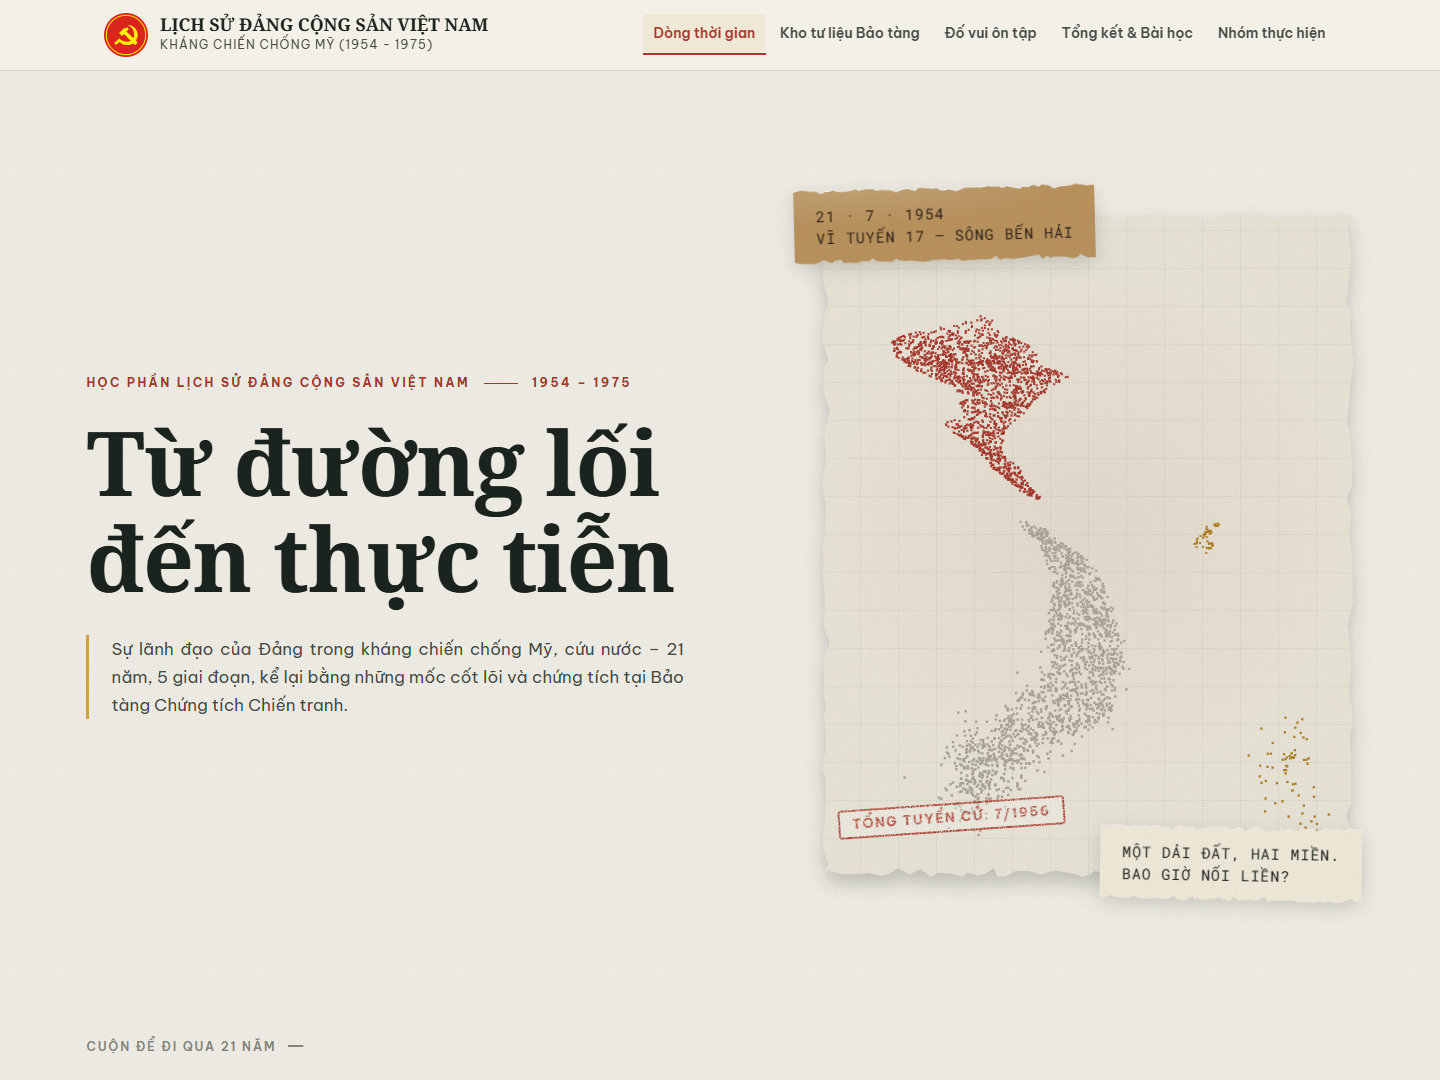
\includegraphics[width=0.94\linewidth,height=0.33\textheight,keepaspectratio]{img/screenshots/hinh-4-01-trang-chu.png}
\caption[Trang mở đầu với chủ đề học liệu và sơ đồ minh họa Việt Nam]{Trang mở đầu với chủ đề học liệu và sơ đồ minh họa Việt Nam. Nguồn: website của nhóm, chụp ngày 23/11/2026.}
\label{fig:web-1}
\end{figure}

\section{Kiến trúc và công nghệ sử dụng}

Website được tổ chức theo kiến trúc giao diện tĩnh, sử dụng \textbf{HTML5, CSS3 và JavaScript thuần}. HTML tạo cấu trúc nội dung; CSS quy định bố cục, màu sắc, kiểu chữ và cách hiển thị trên các kích thước màn hình; JavaScript xử lý điều hướng, dựng nội dung từ dữ liệu, mở hộp chi tiết, dựng và duyệt kho tư liệu, chấm điểm trắc nghiệm. Các khu vực dùng chung một trang HTML và chuyển đổi bằng thao tác điều hướng, không cần tải lại toàn bộ trang cho từng chức năng.

Mã JavaScript của bản triển khai được chia theo trách nhiệm. Tệp {\small\texttt{data.js}} chứa dữ liệu tư liệu bảo tàng, tổng kết và nhóm; {\small\texttt{quiz-data.js}} chứa câu hỏi ôn tập; nội dung dòng thời gian được cung cấp bởi {\small\texttt{timeline-data.js}} thông qua {\small\texttt{TL\_DATA}}; {\small\texttt{timeline.js}}, {\small\texttt{gallery.js}}, {\small\texttt{summary.js}} và {\small\texttt{quiz.js}} xử lý các khu vực tương ứng; {\small\texttt{main.js}} điều phối điều hướng và thông tin nhóm. Tệp {\small\texttt{land3d.js}} tạo hiệu ứng sơ đồ Việt Nam bằng hệ thống điểm hạt trên Canvas 2D, gợi cảm giác chiều sâu và chuyển động. Đây là sơ đồ minh họa cho trải nghiệm học tập, không phải bản đồ địa lý dùng để đo đạc. Các tệp được nạp bằng thẻ {\small\texttt{script}} thông thường; việc chia chức năng không đồng nghĩa với sử dụng chuẩn ES module.

Việc tách dữ liệu khỏi phần xử lý giúp nhóm có thể hiệu đính nội dung, bổ sung hình ảnh hoặc điều chỉnh câu hỏi mà không phải viết lại toàn bộ giao diện. Website hiện xử lý hoạt động học tập ở phía trình duyệt; chưa có hệ thống tài khoản, cơ sở dữ liệu phía máy chủ hay cơ chế lưu kết quả cá nhân lâu dài. Phạm vi này phù hợp với một sản phẩm học liệu trong học phần, tập trung vào truy cập, đọc và ôn tập.

\section{Các chức năng đã hoàn thành}

\subsection{Dòng thời gian tương tác theo năm giai đoạn}

Khu vực Dòng thời gian là trục chính của website. Phiên bản đã triển khai trình bày nội dung theo hình thức \textbf{cuộn kể chuyện kết hợp các khối kiến thức}, thay cho việc chỉ chuyển từng slide riêng biệt. Năm giai đoạn được nối tiếp từ 1954 - 1960 đến 1973 - 1975; mỗi giai đoạn làm rõ bối cảnh, đường lối, kết quả thực tiễn, chứng tích liên quan và nội dung ghi nhớ.

Trên màn hình máy tính, bảng thông tin bên cạnh nội dung hiển thị thời điểm, tên giai đoạn và sơ đồ minh họa. Thước thời gian cho phép chọn nhanh giai đoạn; các ký hiệu phân biệt \textbf{bối cảnh}, \textbf{đường lối} và \textbf{thực tiễn} giúp người đọc nhận ra vai trò của từng mốc. Khi cuộn trang, thông tin đang được theo dõi được cập nhật, hỗ trợ định vị sự kiện trong tiến trình chung. Người dùng cũng có thể chuyển mốc bằng phím mũi tên trái, phải.

\begin{figure}[H]
\centering
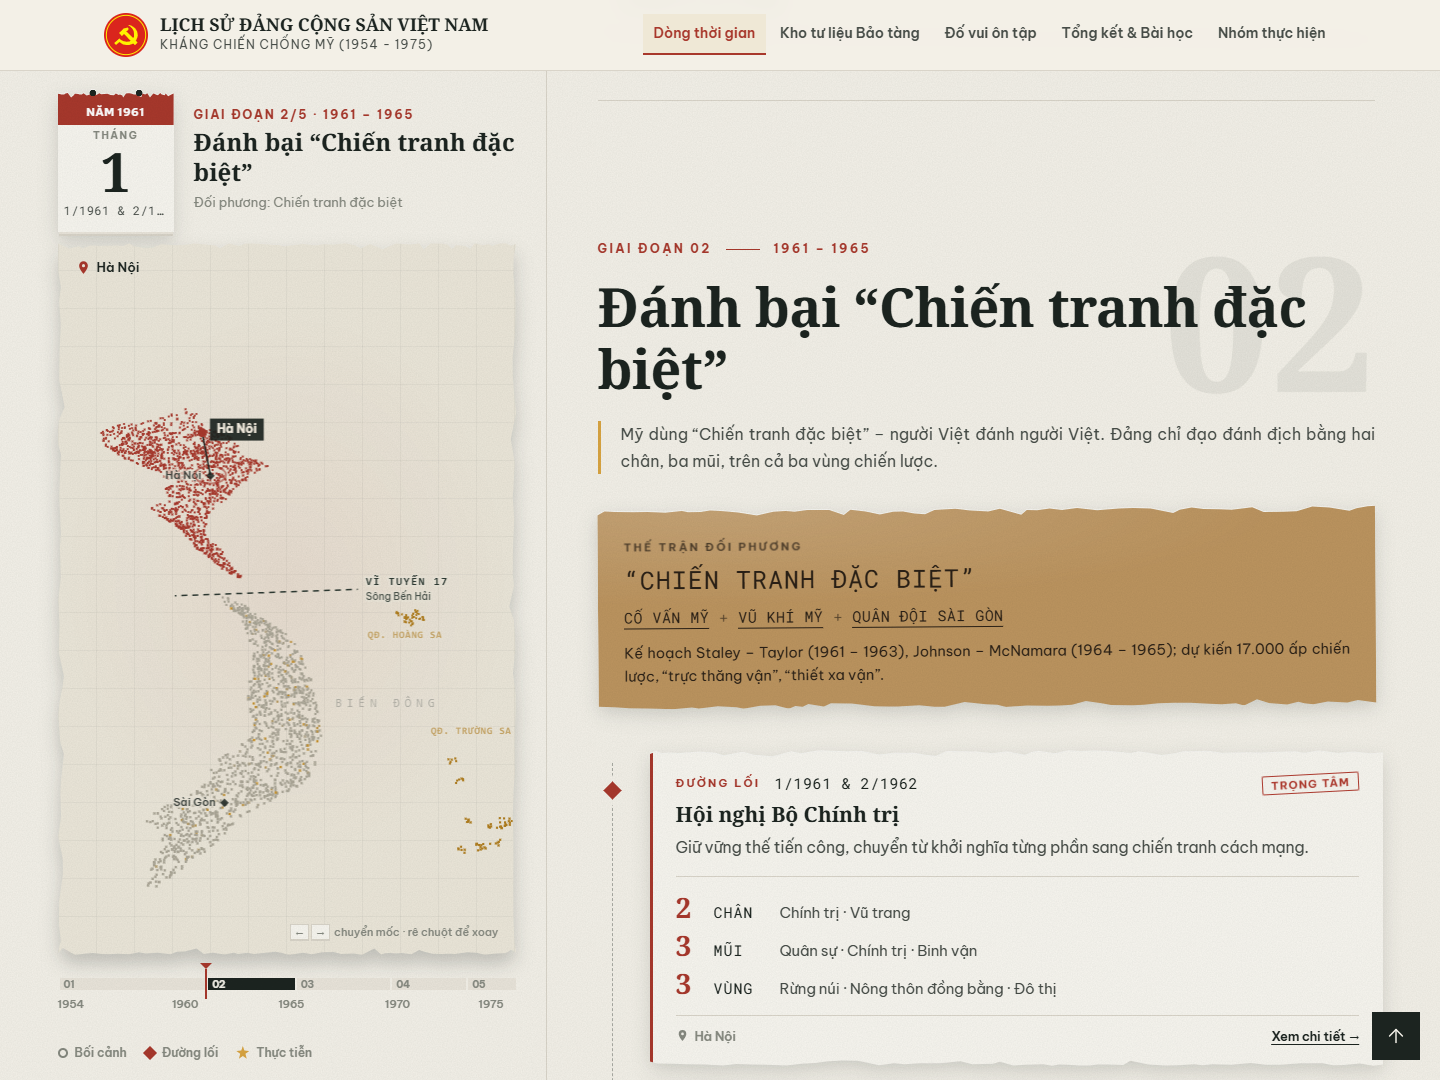
\includegraphics[width=0.94\linewidth,height=0.33\textheight,keepaspectratio]{img/screenshots/hinh-4-02-dong-thoi-gian.png}
\caption[Giai đoạn 1961 - 1965 với bảng thông tin, sơ đồ minh họa và thước thời gian]{Giai đoạn 1961 - 1965 với bảng thông tin, sơ đồ minh họa và thước thời gian. Nguồn: website của nhóm, chụp ngày 23/11/2026.}
\label{fig:web-2}
\end{figure}

Một số mốc trọng tâm có nút \textbf{Xem chi tiết}, mở hộp nội dung bổ sung mà không rời khỏi mạch đọc. Chẳng hạn, người học có thể mở phần Chiến thắng Ấp Bắc để tìm hiểu thêm ý nghĩa thực tiễn của sự kiện. Cách trình bày theo lớp giúp giữ phần tổng quan ngắn gọn, đồng thời dành chỗ cho việc tìm hiểu sâu khi cần.

\begin{figure}[H]
\centering
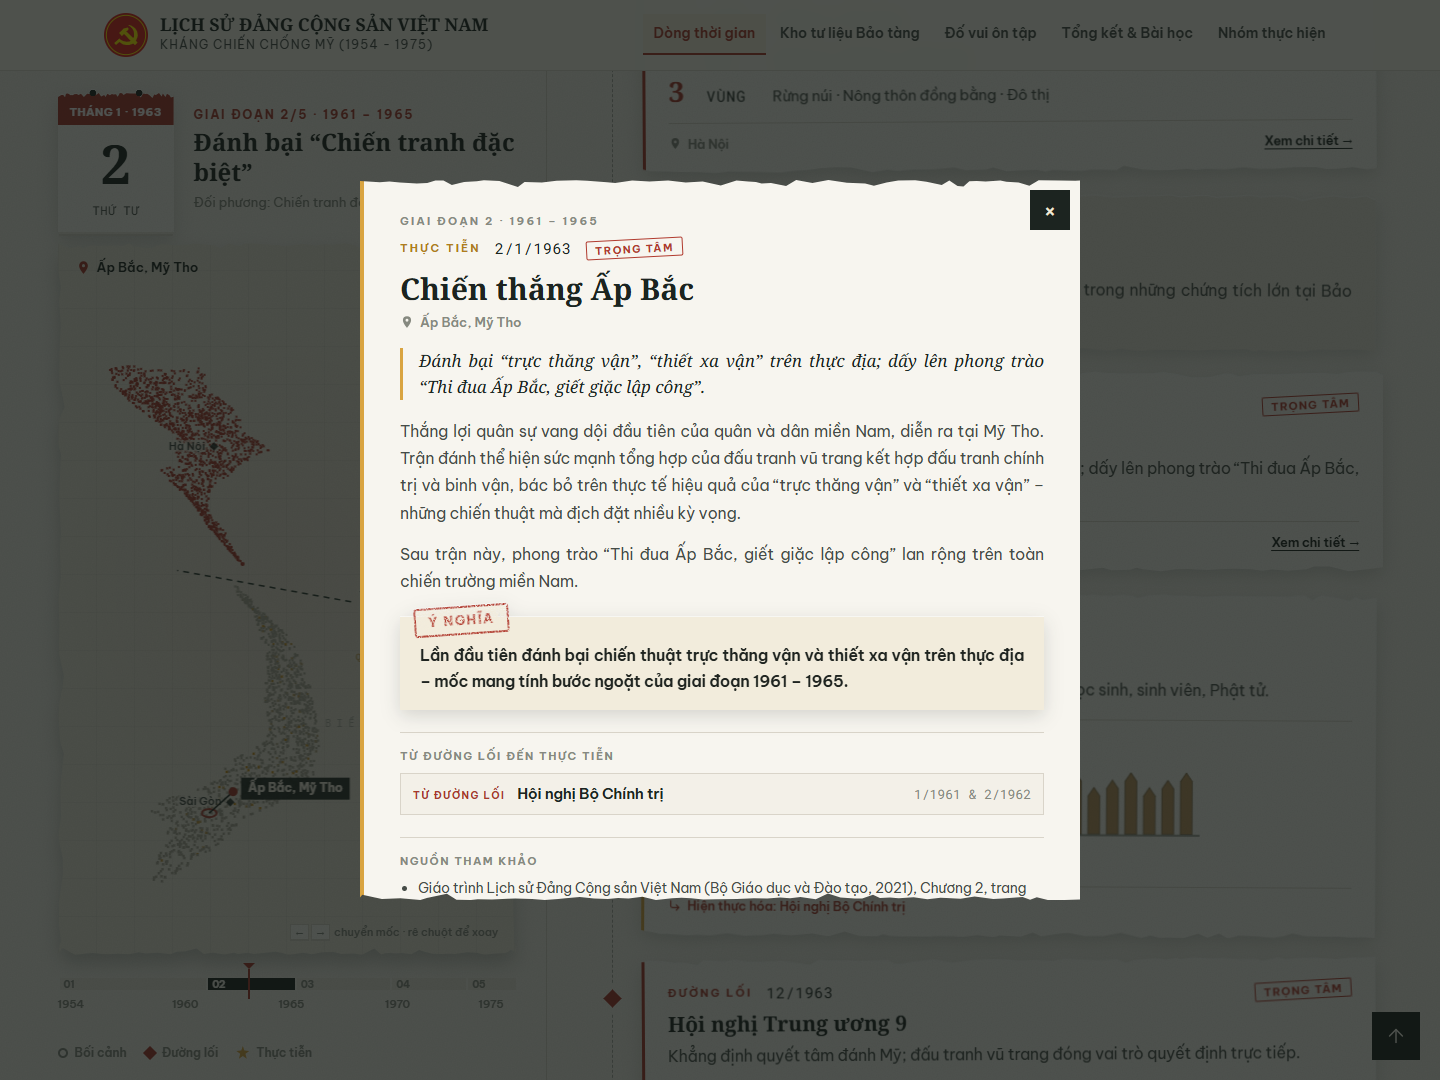
\includegraphics[width=0.94\linewidth,height=0.33\textheight,keepaspectratio]{img/screenshots/hinh-4-03-chi-tiet-su-kien.png}
\caption[Hộp chi tiết sự kiện được mở từ dòng thời gian]{Hộp chi tiết sự kiện được mở từ dòng thời gian. Nguồn: website của nhóm, chụp ngày 23/11/2026.}
\label{fig:web-3}
\end{figure}

\subsection{Kho tư liệu Bảo tàng}

Kho tư liệu tập hợp 13 mục minh họa gắn với năm giai đoạn nghiên cứu. Các thẻ có hình ảnh, tên tư liệu, nhãn giai đoạn và phần giới thiệu ngắn, được trình bày trên cùng một kho để người học duyệt nội dung. Thẻ trực thăng UH-1 Huey được làm nổi bật trên một hàng riêng, kết hợp ảnh lớn với phần thuyết minh và nút liên kết tới dòng thời gian. Cách bố trí này giúp liên hệ hiện vật với bối cảnh và nội dung học liệu mà không cần rời khỏi website.

\begin{figure}[H]
\centering
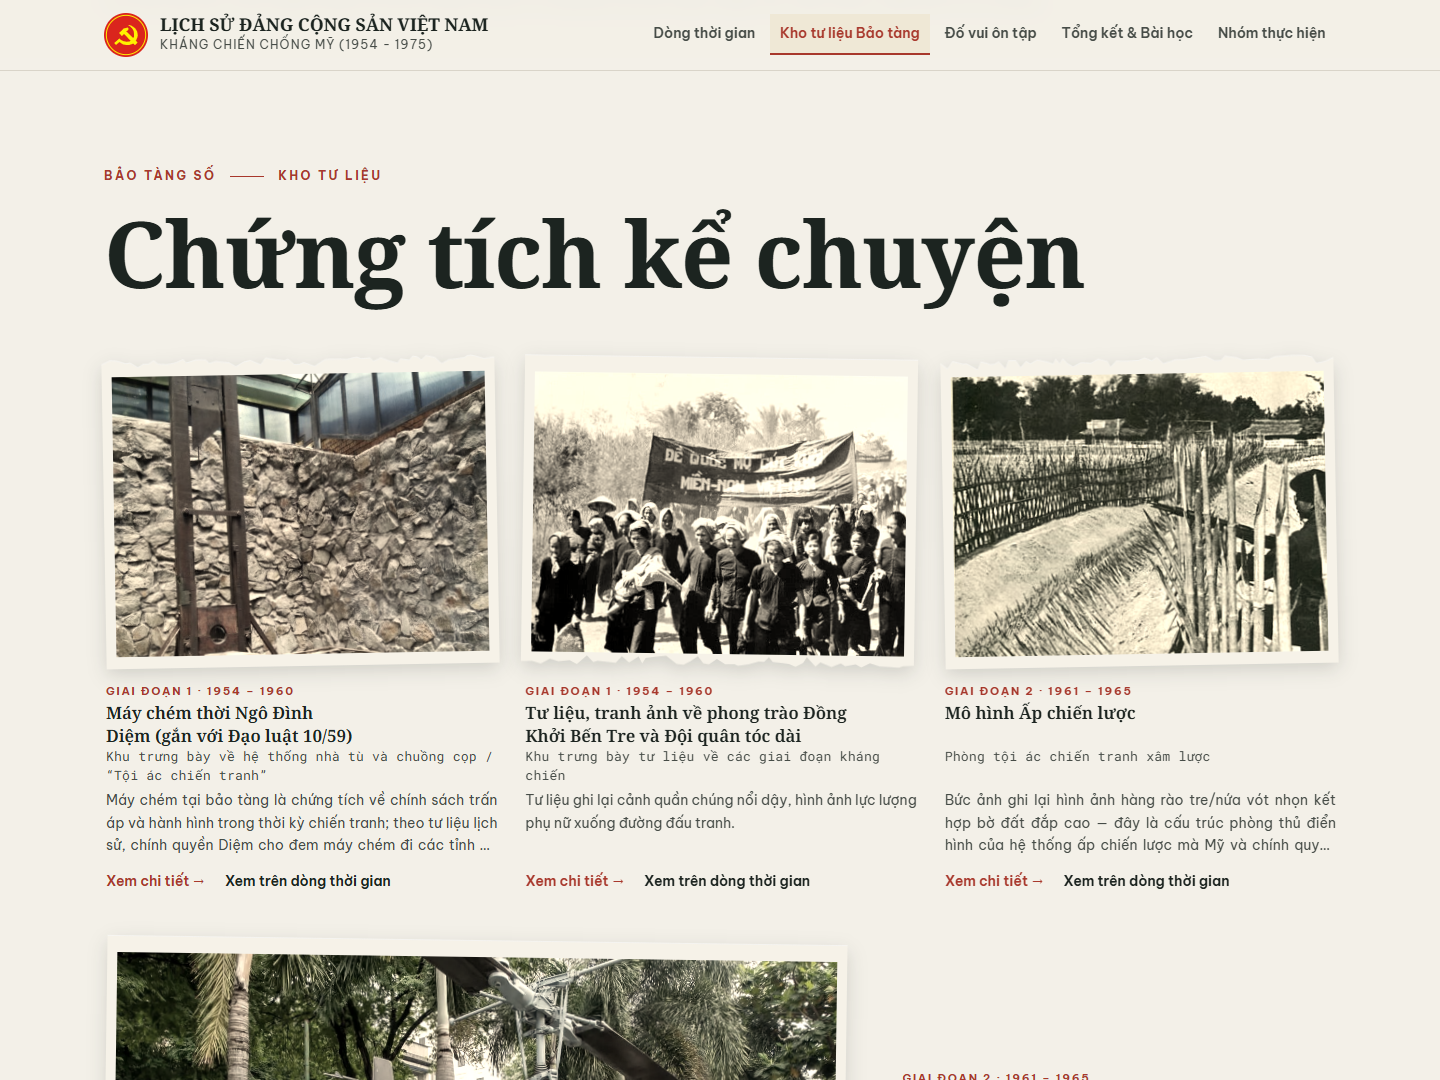
\includegraphics[width=0.94\linewidth,height=0.33\textheight,keepaspectratio]{img/screenshots/hinh-4-04-kho-tu-lieu.png}
\caption[Giao diện kho tư liệu Bảo tàng]{Giao diện kho tư liệu Bảo tàng. Nguồn: website của nhóm, chụp ngày 23/11/2026.}
\label{fig:web-4}
\end{figure}

\begin{figure}[H]
\centering
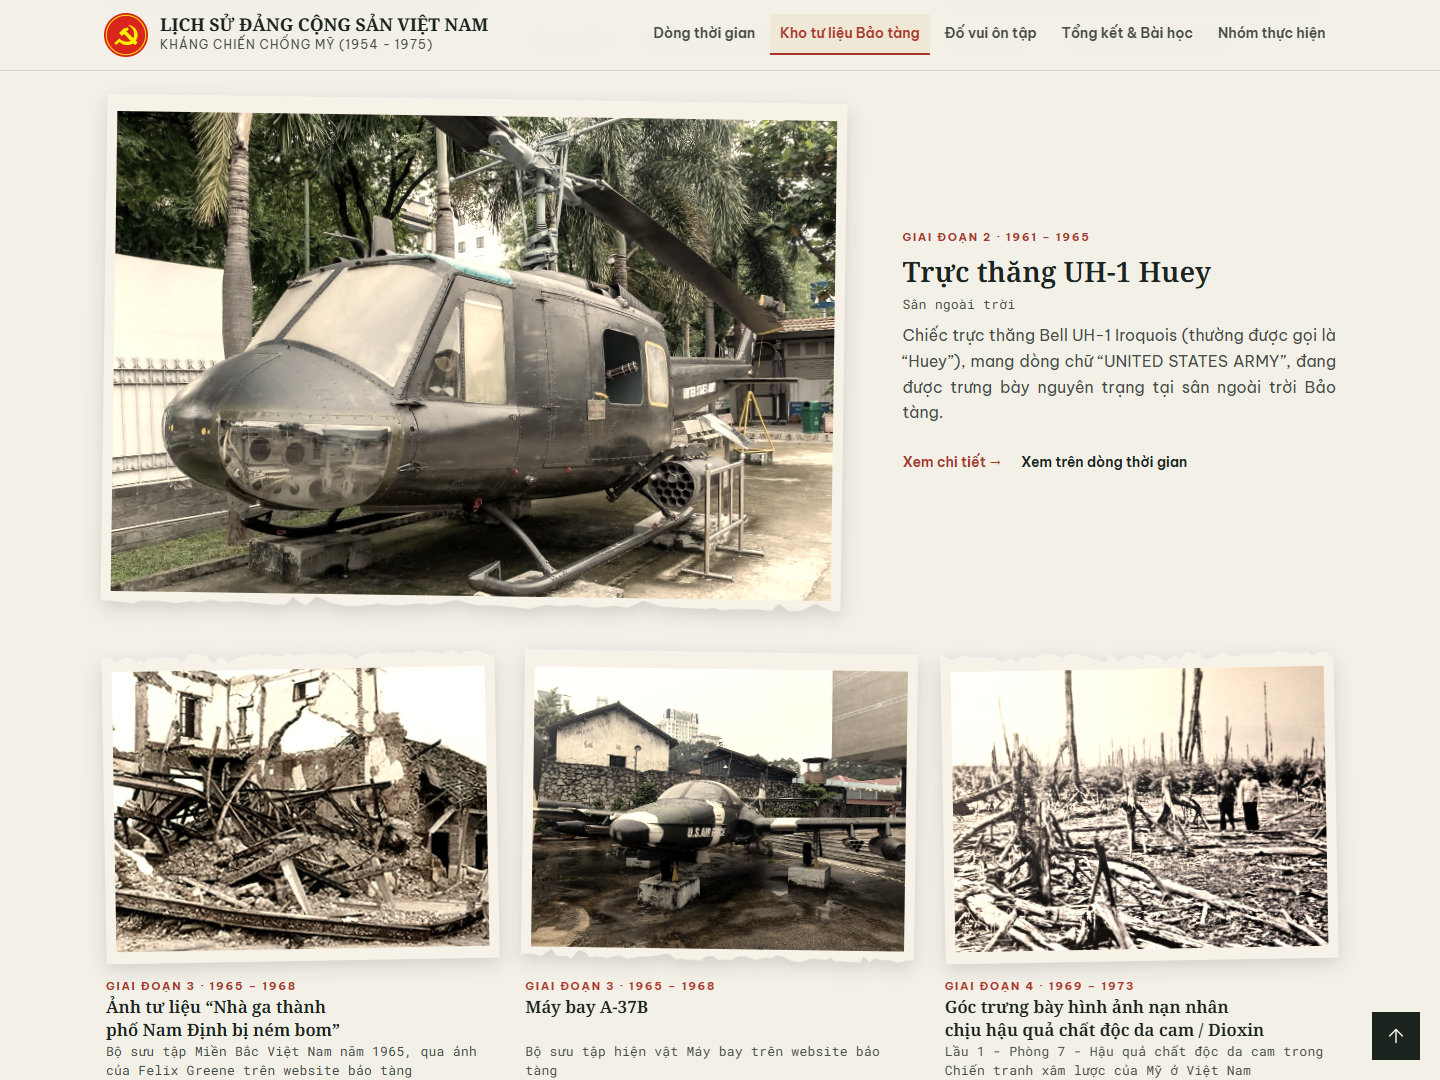
\includegraphics[width=0.94\linewidth,height=0.33\textheight,keepaspectratio]{img/screenshots/hinh-4-05-tu-lieu-noi-bat.png}
\caption[Thẻ trực thăng UH-1 Huey nổi bật và liên kết tới dòng thời gian]{Thẻ trực thăng UH-1 Huey nổi bật và liên kết tới dòng thời gian. Nguồn: website của nhóm, chụp ngày 23/11/2026.}
\label{fig:web-5}
\end{figure}

Nút \textbf{Xem chi tiết} mở ảnh lớn cùng thông tin về vị trí hoặc bộ sưu tập, nội dung thuyết minh và nhãn nguồn ảnh. Hộp chi tiết có điều hướng giữa các mục và nút \textbf{Xem trên dòng thời gian}, giúp đưa tư liệu trở lại bối cảnh lịch sử liên quan. Hình 4.6 minh họa trực thăng UH-1 Huey với phần ghi nhận nguồn ảnh do nhóm sinh viên chụp. Website sử dụng cả ảnh nhóm chụp và ảnh từ Internet; vì vậy, cần xem nhãn nguồn của từng mục thay vì coi toàn bộ hình ảnh đều là ảnh khảo sát của nhóm.

\begin{figure}[H]
\centering
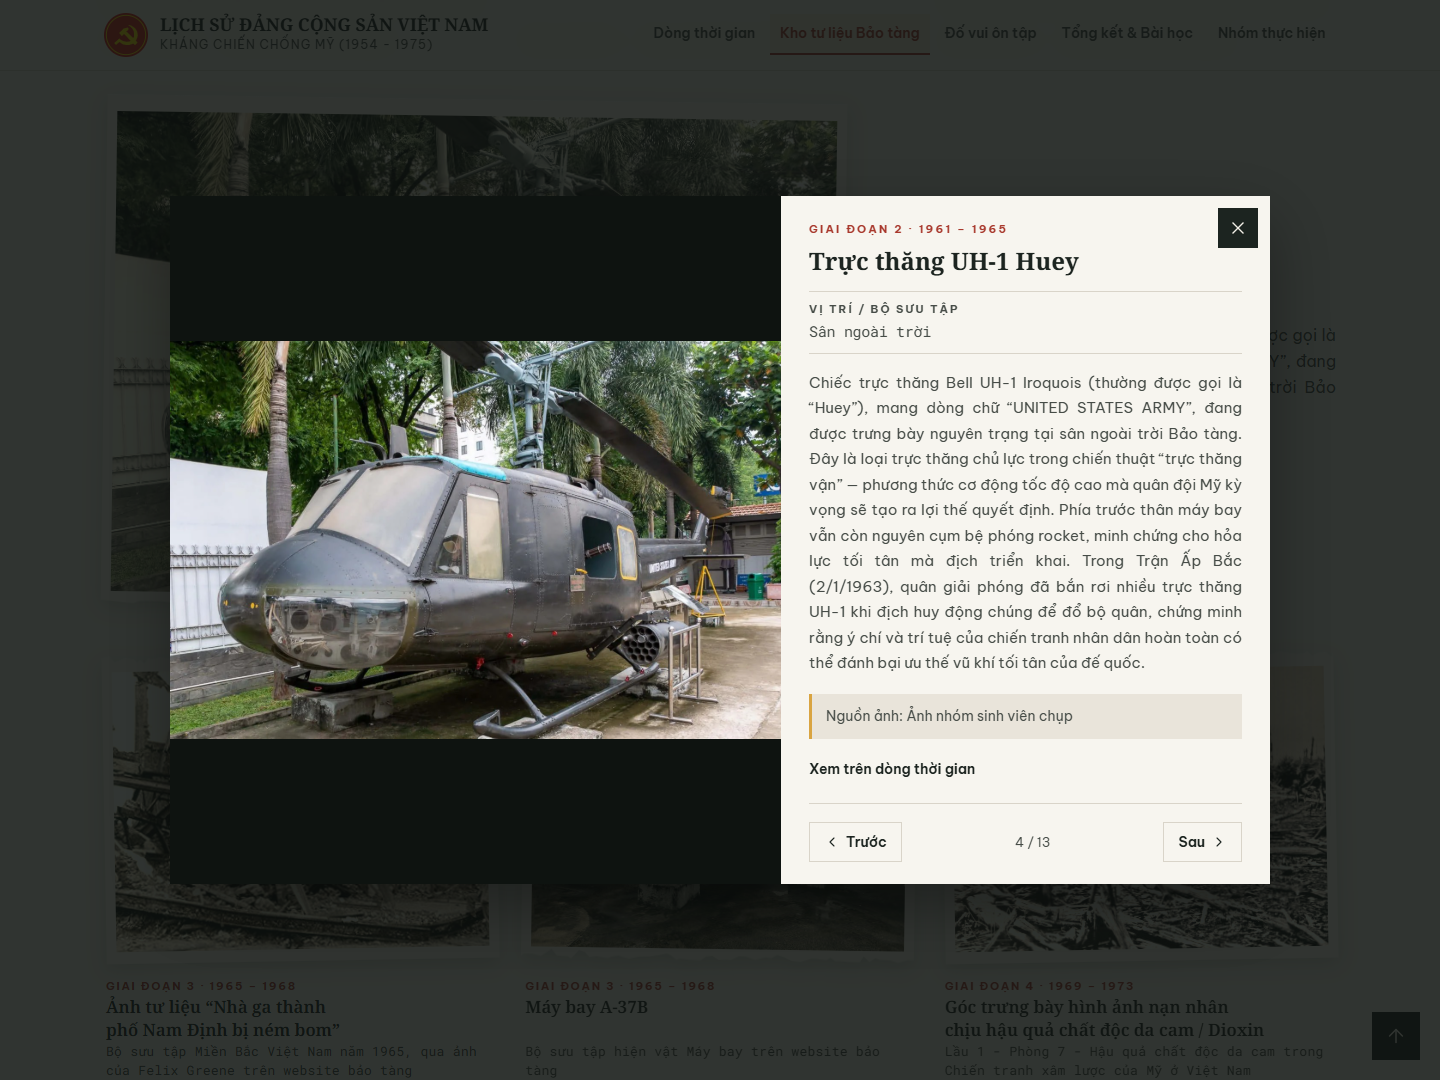
\includegraphics[width=0.94\linewidth,height=0.33\textheight,keepaspectratio]{img/screenshots/hinh-4-06-chi-tiet-tu-lieu.png}
\caption[Ảnh phóng lớn, thuyết minh và nguồn tư liệu của trực thăng UH-1 Huey]{Ảnh phóng lớn, thuyết minh và nguồn tư liệu của trực thăng UH-1 Huey. Nguồn: website của nhóm, chụp ngày 23/11/2026.}
\label{fig:web-6}
\end{figure}

Giá trị của kho tư liệu không chỉ nằm ở khả năng xem ảnh. Việc đặt chú thích và thông tin lịch sử cạnh hình ảnh giúp người học đặt câu hỏi: tư liệu phản ánh vấn đề gì, thuộc bối cảnh nào và có thể minh họa cho luận điểm nào trong giáo trình. Đây là sự tiếp nối phương pháp đối chiếu giữa đường lối và thực tiễn đã trình bày ở phần 1.

\subsection{Trắc nghiệm ôn tập có phản hồi giải thích}

Phần Đố vui ôn tập gồm \textbf{19 câu hỏi trắc nghiệm}, xoay quanh các nghị quyết, chủ trương và sự kiện trọng tâm. Mỗi câu có bốn phương án, chỉ chọn một đáp án. Giao diện hiển thị thời kỳ, số thứ tự câu, điểm hiện tại và thanh tiến độ để người học theo dõi quá trình làm bài.

\begin{figure}[H]
\centering
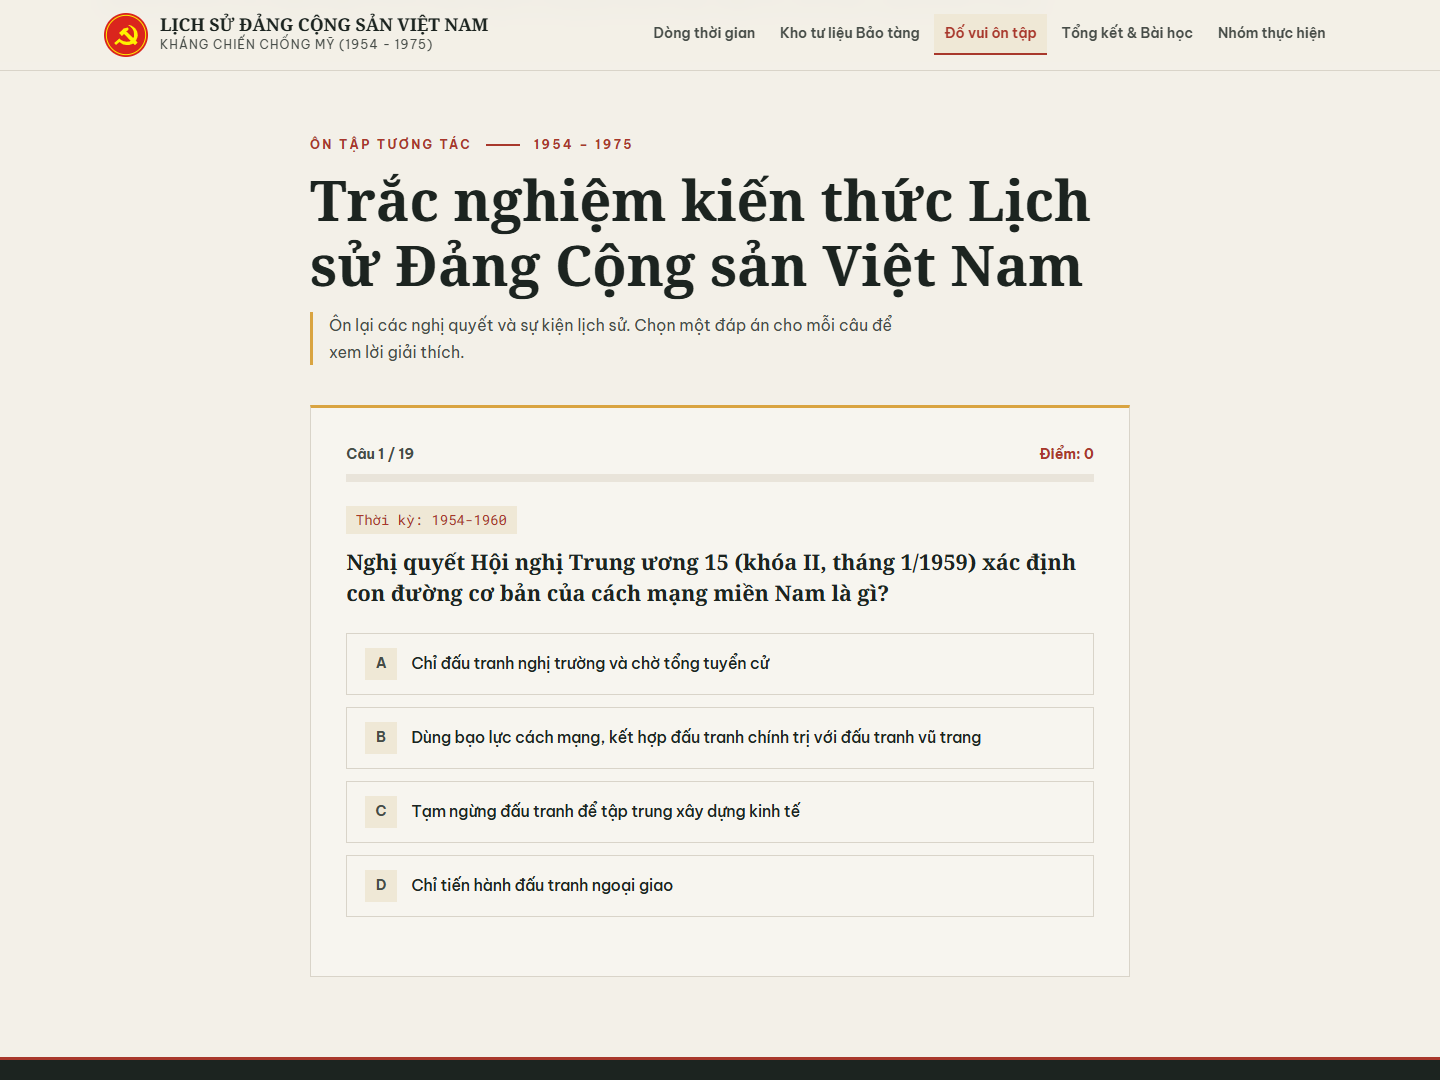
\includegraphics[width=0.94\linewidth,height=0.33\textheight,keepaspectratio]{img/screenshots/hinh-4-07-cau-hoi-on-tap.png}
\caption[Câu đầu tiên trong bộ 19 câu hỏi ôn tập]{Câu đầu tiên trong bộ 19 câu hỏi ôn tập. Nguồn: website của nhóm, chụp ngày 23/11/2026.}
\label{fig:web-7}
\end{figure}

Sau khi chọn, các phương án được khóa để tránh thay đổi hoặc tính điểm lặp lại. Hệ thống đánh dấu đáp án đúng; nếu chọn sai, phương án đã chọn được phân biệt với đáp án đúng và có thông báo bằng chữ. Phần giải thích xuất hiện ngay sau đó, giúp người học nhận biết căn cứ của đáp án trước khi chuyển câu. Như vậy, bài ôn tập không chỉ trả về điểm số mà còn cung cấp phản hồi để sửa nhận thức chưa chính xác.

\begin{figure}[H]
\centering
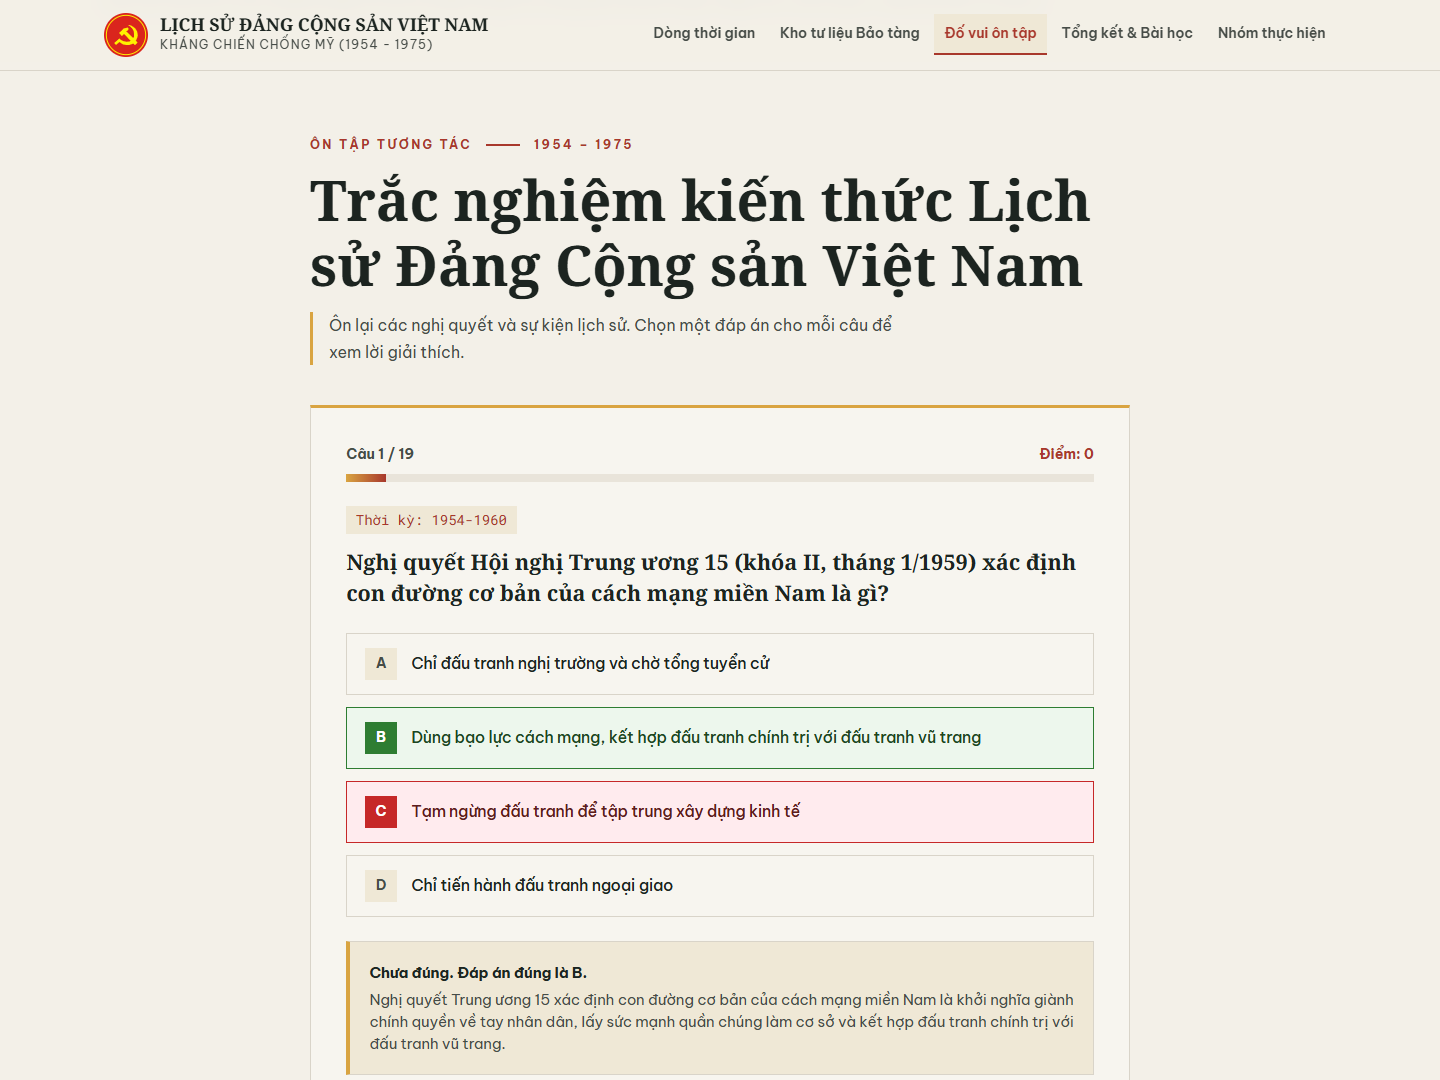
\includegraphics[width=0.94\linewidth,height=0.33\textheight,keepaspectratio]{img/screenshots/hinh-4-08-phan-hoi-dap-an.png}
\caption[Lựa chọn sai được phân biệt với đáp án đúng, kèm giải thích]{Lựa chọn sai được phân biệt với đáp án đúng, kèm giải thích. Nguồn: website của nhóm, chụp ngày 23/11/2026.}
\label{fig:web-8}
\end{figure}

Khi hoàn thành, website hiển thị số câu đúng trên tổng số câu và nhận xét tương ứng. Trong lượt thao tác minh họa, câu đầu được cố ý chọn sai và 18 câu còn lại chọn đúng; hệ thống trả về \textbf{18/19}, phù hợp với cách tính một điểm cho mỗi câu đúng. Đây là kết quả kiểm tra chức năng của một lượt chạy, không phải số liệu khảo sát người học hay bằng chứng đo lường hiệu quả đào tạo.

\begin{figure}[H]
\centering
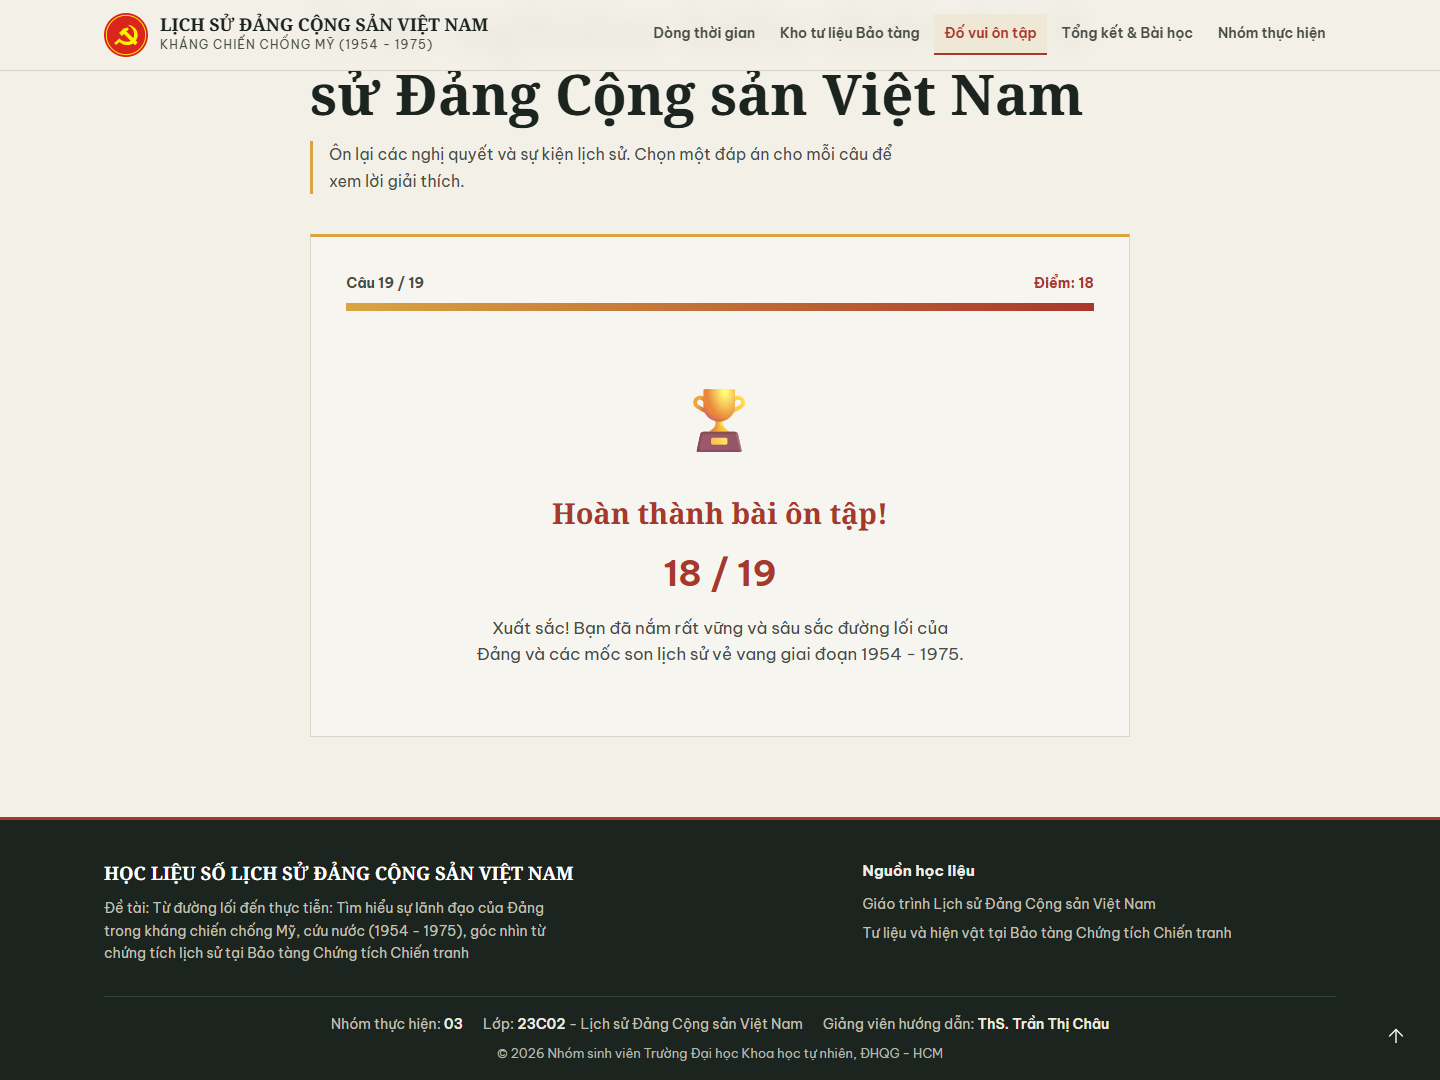
\includegraphics[width=0.94\linewidth,height=0.33\textheight,keepaspectratio]{img/screenshots/hinh-4-09-ket-qua-on-tap.png}
\caption[Màn hình kết quả của lượt kiểm tra minh họa 18/19]{Màn hình kết quả của lượt kiểm tra minh họa 18/19. Nguồn: website của nhóm, chụp ngày 23/11/2026.}
\label{fig:web-9}
\end{figure}

\subsection{Tổng kết và bài học kinh nghiệm}

Khu vực Tổng kết \& Bài học giúp người học chuyển từ theo dõi từng giai đoạn sang khái quát toàn bộ tiến trình. Nội dung bao gồm đánh giá vai trò lãnh đạo của Đảng, bốn nguyên nhân thắng lợi, ý nghĩa lịch sử và năm bài học kinh nghiệm. Mục lục bên cạnh hỗ trợ chuyển nhanh giữa các chủ đề; phần cuối có liên kết sang hoạt động ôn tập.

\begin{figure}[H]
\centering
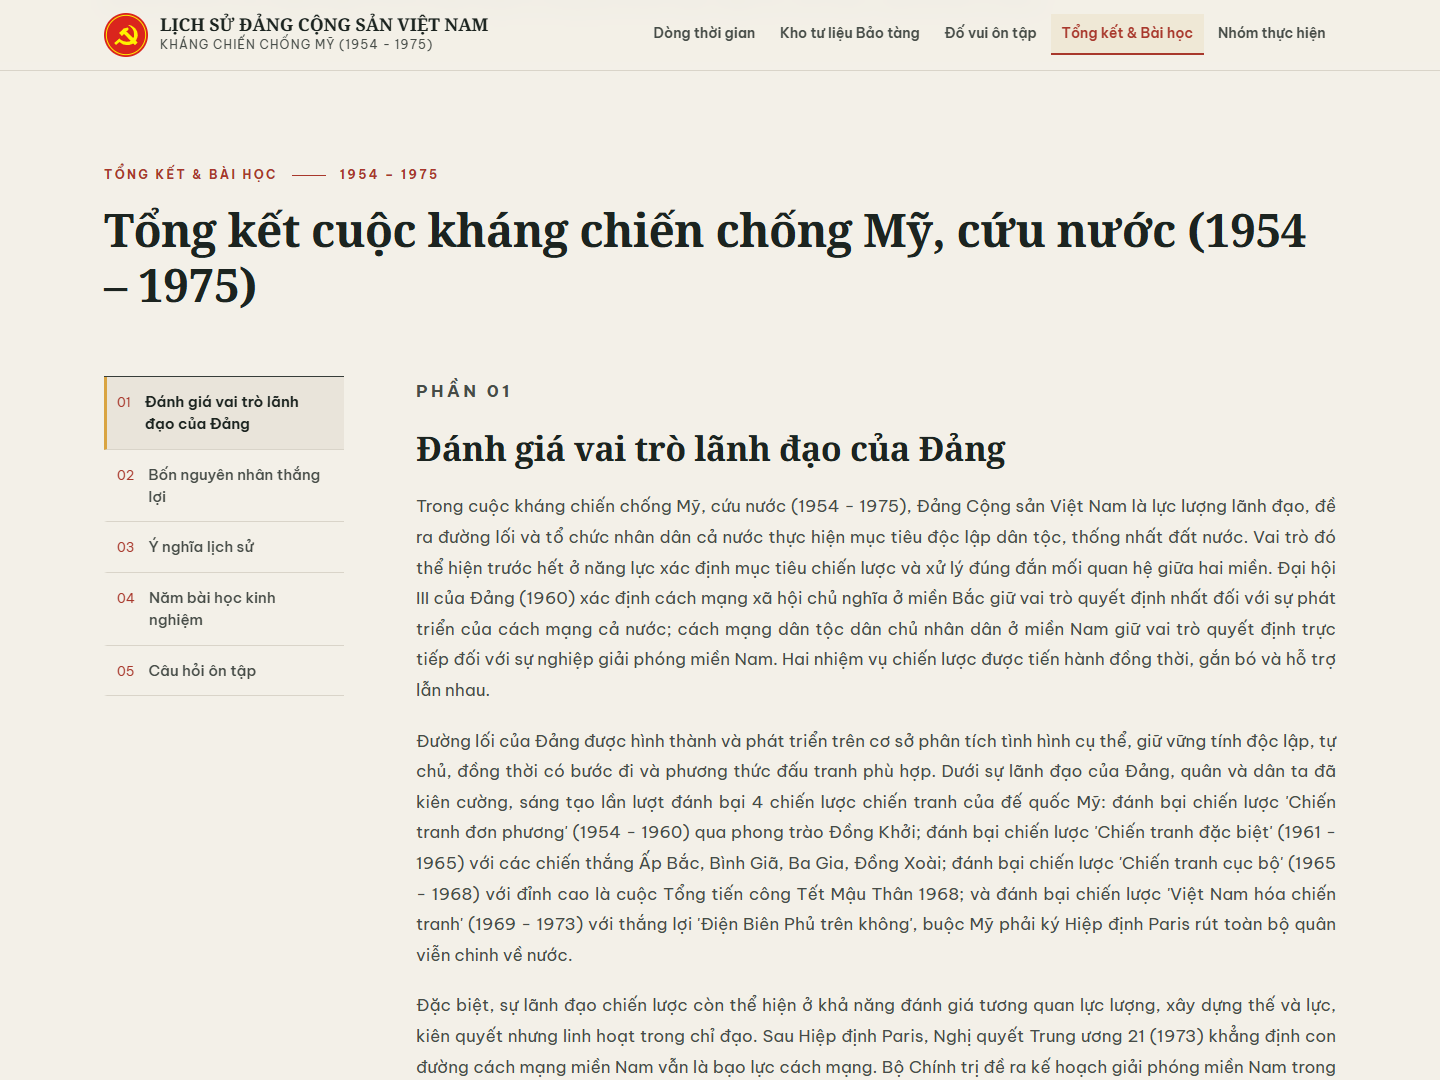
\includegraphics[width=0.94\linewidth,height=0.33\textheight,keepaspectratio]{img/screenshots/hinh-4-10-tong-ket-bai-hoc.png}
\caption[Khu vực tổng kết với mục lục điều hướng theo chủ đề]{Khu vực tổng kết với mục lục điều hướng theo chủ đề. Nguồn: website của nhóm, chụp ngày 23/11/2026.}
\label{fig:web-10}
\end{figure}

Chức năng này gắn với nội dung phần 3 của báo cáo: các sự kiện không được xem như những mốc rời rạc mà là cơ sở để nhận diện quan hệ giữa mục tiêu chiến lược, phương pháp đấu tranh, sức mạnh nhân dân và tổ chức thực hiện. Việc bố trí phần tổng kết ngay trên website tạo điều kiện đối chiếu giữa kiến thức chi tiết và nhận định khái quát.

\subsection{Giới thiệu nhóm và hiển thị trên thiết bị di động}

Trang Nhóm thực hiện giới thiệu tập thể nhóm 03, lớp 23C02, gồm 10 thành viên. Thông tin thành viên gắn với vai trò và nhiệm vụ, từ biên soạn nội dung, xây dựng giao diện và chức năng đến điều phối, tổng hợp báo cáo. Ảnh tập thể tại bảo tàng bổ sung dấu ấn của quá trình khảo sát thực tế.

\begin{figure}[H]
\centering
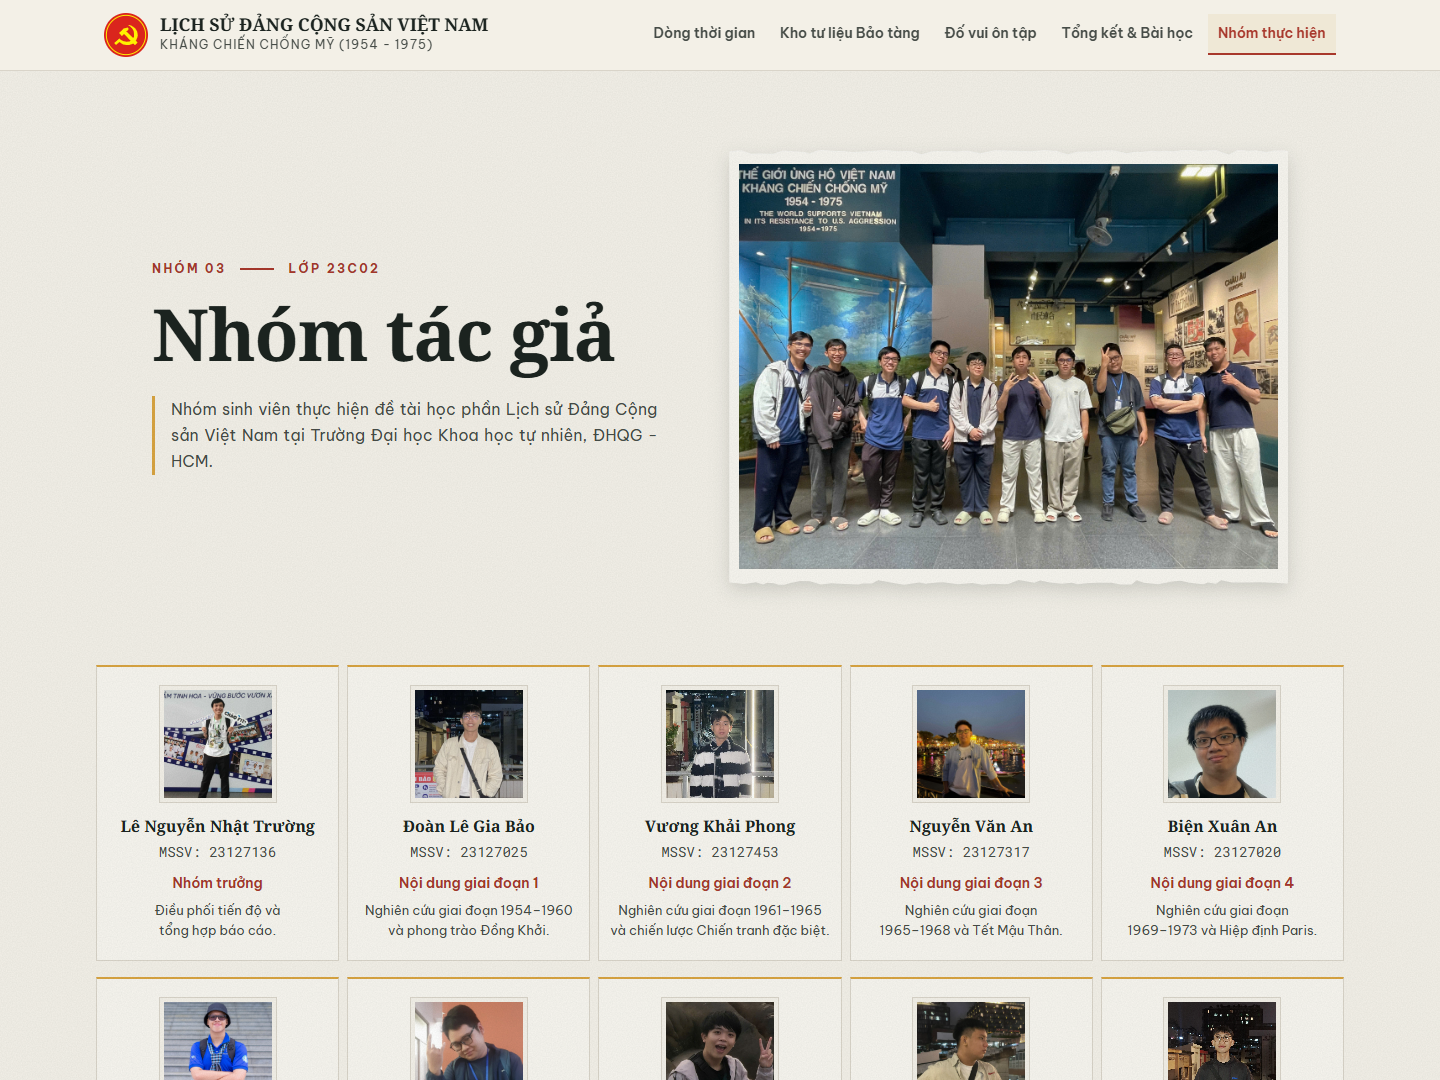
\includegraphics[width=0.94\linewidth,height=0.33\textheight,keepaspectratio]{img/screenshots/hinh-4-12-nhom-thuc-hien.png}
\caption[Trang nhóm tác giả với ảnh tập thể và các thẻ thành viên]{Trang nhóm tác giả với ảnh tập thể và các thẻ thành viên. Nguồn: website của nhóm, chụp ngày 23/11/2026.}
\label{fig:web-11}
\end{figure}

Giao diện có điều chỉnh bố cục theo kích thước màn hình và menu thu gọn trên thiết bị di động. Khi kiểm tra trên \textbf{giao diện điện thoại}, menu mở và chuyển được sang phần Đố vui ôn tập; nội dung trang không gây tràn ngang. Kết quả này xác nhận thao tác cơ bản ở một kích thước màn hình, chưa đại diện cho mọi thiết bị và trình duyệt.

\begin{figure}[H]
\centering
\begin{subfigure}[t]{0.27\textwidth}
\centering

\includegraphics[width=\linewidth]{img/screenshots/hinh-4-13-giao-dien-di-dong.png}
\caption{Phần đầu bài ôn tập}
\end{subfigure}\hspace{0.06\textwidth}%
\begin{subfigure}[t]{0.27\textwidth}
\centering
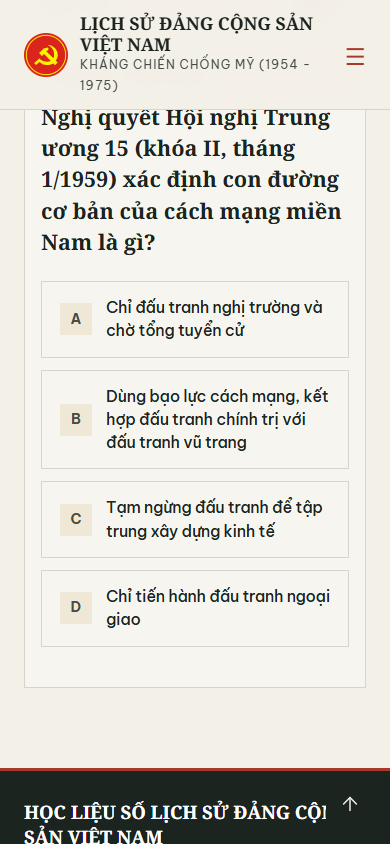
\includegraphics[width=\linewidth]{img/screenshots/hinh-4-14-giao-dien-di-dong-cuon.png}
\caption{Phần dưới sau khi cuộn}
\end{subfigure}
\caption[Giao diện ôn tập trên điện thoại]{Giao diện điện thoại: phần đầu bài ôn tập và phần dưới sau khi cuộn. Nguồn: website của nhóm, chụp ngày 23/11/2026.}
\label{fig:web-12}
\end{figure}

\section{Đánh giá kết quả và khả năng ứng dụng}

\subsection{Kết quả kiểm tra các thao tác chính}

Việc kiểm tra được thực hiện trực tiếp trên bản đã triển khai bằng trình duyệt Microsoft Edge ngày 23/11/2026, với khung nhìn máy tính 1440 × 1080 pixel và khung nhìn di động nêu trên. Các kết quả dưới đây phản ánh phạm vi thao tác đã kiểm tra, không thay thế một đợt đánh giá toàn diện về hiệu năng, bảo mật hoặc khả năng tiếp cận.

\begin{table}[H]
\centering
\begingroup\small\setstretch{1.1}\renewcommand{\arraystretch}{1.25}\setlength{\extrarowheight}{2pt}
\begin{tabularx}{\textwidth}{|>{\raggedright\arraybackslash}p{0.33\textwidth}|L|}
\hline
\textbf{Thao tác kiểm tra} & \textbf{Kết quả ghi nhận} \\
\hline
Truy cập địa chỉ triển khai & Trang phản hồi HTTP 200 và hiển thị nội dung \\
\hline
Chọn giai đoạn trên thước thời gian & Chuyển đến nội dung giai đoạn 1961 - 1965 \\
\hline
Mở chi tiết sự kiện & Hiển thị nội dung Chiến thắng Ấp Bắc; đóng được bằng phím Escape \\
\hline
Duyệt kho tư liệu và thẻ nổi bật & Hiển thị 13 mục có nhãn giai đoạn; trực thăng UH-1 Huey được làm nổi bật \\
\hline
Mở chi tiết tư liệu & Hiển thị ảnh, thuyết minh và nguồn; đóng được bằng phím Escape \\
\hline
Trả lời trắc nghiệm & Có phản hồi, giải thích và khóa bốn lựa chọn sau khi trả lời \\
\hline
Hoàn thành toàn bộ 19 câu & Lượt minh họa 18 câu đúng, 1 câu sai trả về 18/19 \\
\hline
Chọn mục Năm bài học kinh nghiệm & Chuyển đến phần tương ứng trong khu vực tổng kết \\
\hline
Điều hướng trên khung nhìn di động & Menu thu gọn hoạt động, mở được phần ôn tập \\
\hline
\end{tabularx}
\endgroup
\caption{Kết quả kiểm tra các thao tác chính trên website}
\label{tab:web-2}
\end{table}

\subsection{Giá trị hỗ trợ học tập}

Website tạo một lộ trình có thể sử dụng khi tự học: \textbf{đọc tiến trình \ensuremath{\rightarrow} xem tư liệu liên quan \ensuremath{\rightarrow} tổng hợp kiến thức \ensuremath{\rightarrow} trả lời câu hỏi \ensuremath{\rightarrow} đọc giải thích và xem lại nội dung}. Người học được lựa chọn điểm bắt đầu theo nhu cầu, còn các giai đoạn và mục lục giúp duy trì định hướng. Trong thảo luận nhóm, dòng thời gian và hộp chi tiết có thể được dùng để minh họa luận điểm, kết hợp với phần thuyết trình của sinh viên.

So với tập hợp tài liệu rời, sản phẩm có ưu điểm là đặt nội dung nghiên cứu, hình ảnh và ôn tập trong một môi trường truy cập chung. Tuy nhiên, giá trị hiện được xác định ở khả năng tổ chức và hỗ trợ hoạt động học tập; nhóm chưa có khảo sát đủ cơ sở để kết luận website làm tăng điểm số hoặc mức độ ghi nhớ. Giáo trình và hướng dẫn của giảng viên vẫn là nền tảng học thuật, còn điểm trắc nghiệm chỉ phục vụ tự kiểm tra.

\subsection{Hạn chế và hướng phát triển}

Phạm vi học liệu và bộ 19 câu hỏi còn giới hạn, chưa bao quát toàn bộ yêu cầu của học phần. Nguồn ảnh và thuyết minh cần tiếp tục được rà soát, đặc biệt là việc phân biệt ảnh hiện vật, ảnh tư liệu và hình minh họa; trích nguồn không thay thế yêu cầu tuân thủ quyền sử dụng hình ảnh. Những hiệu ứng chuyển động cũng cần được kiểm tra thêm trên thiết bị cấu hình thấp và với người dùng có nhu cầu tiếp cận khác nhau.

Trong các lần hoàn thiện tiếp theo, nhóm có thể ưu tiên hiệu đính nội dung, chuẩn hóa nguồn trích dẫn, mở rộng câu hỏi theo chủ đề và bổ sung chức năng xem lại câu trả lời sai. Việc lưu tiến độ cá nhân hoặc thống kê kết quả chỉ nên phát triển khi có nhu cầu rõ ràng và phương án bảo vệ dữ liệu phù hợp. Trước mắt, trọng tâm vẫn là độ chính xác của học liệu, tính rõ ràng của giao diện và khả năng sử dụng các chức năng cốt lõi.

\clearpage

% Nội dung báo cáo được chuyển từ bản Markdown đã đối chiếu.
\chapter{KẾT LUẬN VÀ CẢM NGHĨ CỦA NHÓM}

\section{Kết luận}

Đề tài đã kết hợp nghiên cứu lịch sử với việc xây dựng một sản phẩm học liệu số có thể truy cập và sử dụng trên trình duyệt. Phần nội dung hệ thống hóa sự lãnh đạo của Đảng qua năm giai đoạn kháng chiến chống Mỹ, cứu nước; phần sản phẩm chuyển nội dung đó thành dòng thời gian tương tác, kho tư liệu, bài tổng kết và hoạt động trắc nghiệm có giải thích. Website vì vậy là kết quả ứng dụng trực tiếp của quá trình chọn lọc, tổ chức và trình bày tri thức mà nhóm đã thực hiện.

Kết quả nổi bật của nhóm không chỉ là một địa chỉ web được triển khai, mà còn là sự kết nối giữa các hình thức tiếp cận: đọc để nắm tiến trình, quan sát để hình dung chứng tích và tự kiểm tra để nhận ra nội dung cần củng cố. Qua đó, mục tiêu “từ đường lối đến thực tiễn” được thể hiện cả trong nội dung lịch sử lẫn cách tổ chức hoạt động học tập. Những chức năng đã kiểm tra cho thấy sản phẩm đáp ứng các thao tác cơ bản trong phạm vi đề tài; việc đánh giá hiệu quả học tập thực tế cần được tiếp tục bằng phản hồi và khảo sát người sử dụng.

\section{Cảm nghĩ sau quá trình khảo sát và xây dựng sản phẩm}

Qua việc tìm hiểu chứng tích tại Bảo tàng Chứng tích Chiến tranh, nhóm nhận thức rõ hơn rằng các mốc lịch sử trong giáo trình gắn với đời sống, sự hy sinh và những mất mát cụ thể của con người. Các hiện vật, ảnh tư liệu và nội dung trưng bày giúp việc học không dừng lại ở tên gọi của một chiến lược hay kết quả của một chiến dịch. Đằng sau đó là những nỗ lực bền bỉ của nhân dân, sự phối hợp giữa hậu phương và tiền tuyến, cùng khát vọng độc lập, thống nhất và hòa bình.

Những ghi nhận ấy làm sâu sắc lòng biết ơn của nhóm đối với các thế hệ đi trước, đồng thời nhắc nhở trách nhiệm khi chuyển tư liệu thành nội dung số. Một hình ảnh không nên chỉ được dùng để tạo ấn tượng; nó cần có bối cảnh và chú thích phù hợp. Một câu hỏi trắc nghiệm không chỉ cần đáp án đúng mà còn cần giải thích rõ. Với nhóm, thái độ nghiêm túc trong kiểm chứng và trình bày kiến thức cũng là cách thể hiện sự tôn trọng lịch sử và người học.

Quá trình xây dựng website còn cho thấy giá trị của hợp tác. Nội dung, thiết kế và lập trình chỉ tạo thành sản phẩm khi được phối hợp và rà soát cùng nhau. Các thành viên có cơ hội rèn luyện kỹ năng phân công, tổng hợp tài liệu, trao đổi và chịu trách nhiệm đối với phần việc chung. Việc vận dụng công nghệ vào môn học giúp nhóm nhận thấy chuyên môn của sinh viên có thể góp phần làm cho học liệu dễ tiếp cận hơn, nhưng không thay thế yêu cầu nghiên cứu nghiêm túc.

Từ trải nghiệm đó, nhóm xác định trách nhiệm của người trẻ bắt đầu từ những việc cụ thể: học tập có mục tiêu, sử dụng thông tin có kiểm chứng, tôn trọng con người và đóng góp bằng năng lực của mình. Trân trọng hòa bình không chỉ là cảm xúc trước chứng tích chiến tranh mà còn là ý thức gìn giữ, xây dựng cuộc sống hôm nay và ứng xử có trách nhiệm trong cộng đồng.

\section{Lời cảm ơn}

Nhóm xin trân trọng cảm ơn Ban Giám hiệu Trường Đại học Khoa học Tự nhiên, Đại học Quốc gia Thành phố Hồ Chí Minh; quý Thầy, Cô phụ trách học phần Lịch sử Đảng Cộng sản Việt Nam đã tạo điều kiện để sinh viên kết hợp học tập lý luận với tìm hiểu thực tế. Nhóm cảm ơn Bảo tàng Chứng tích Chiến tranh đã gìn giữ, trưng bày và giới thiệu hệ thống tư liệu giúp công chúng tiếp cận lịch sử từ những chứng tích cụ thể.

Nhóm cũng cảm ơn sự phối hợp và đóng góp của các thành viên trong quá trình biên soạn nội dung, khảo sát, xây dựng và hoàn thiện website. Dù đã nỗ lực thực hiện, sản phẩm và báo cáo vẫn có thể còn hạn chế. Nhóm mong nhận được góp ý của giảng viên và người học để tiếp tục hiệu đính, hoàn thiện học liệu theo hướng chính xác, rõ ràng và hữu ích hơn.

\clearpage

\backmatter
\begin{thebibliography}{9}
\addcontentsline{toc}{chapter}{TÀI LIỆU THAM KHẢO}
\bibitem{ref1} Bộ Giáo dục và Đào tạo (2021), \emph{Giáo trình Lịch sử Đảng Cộng sản Việt Nam (Dành cho bậc đại học hệ không chuyên lý luận chính trị)}, Nhà xuất bản Chính trị quốc gia Sự thật, Hà Nội.

\bibitem{ref2} Bảo tàng Chứng tích Chiến tranh, \emph{Bộ sưu tập Máy bay}, \href{https://baotangchungtichchientranh.vn/kham-pha/bo-suu-tap/may-bay}{Cổng thông tin Bảo tàng Chứng tích Chiến tranh}.

\bibitem{ref3} Nhóm 03, lớp 23C02 (2026), \emph{Website học liệu Từ đường lối đến thực tiễn}, \href{https://nhom03-lsd-23c02.vercel.app/}{bản triển khai trên Vercel}, truy cập và chụp màn hình ngày 23/11/2026.
\end{thebibliography}

\end{document}
